%%%%%%%%%%%%%%%%%%%%%%%%%%%%%%%%%%%%%%%%%%%%%%%%%%%%%%%%%%%%%%%%%%%%%%%%%%%%%%%%%%%
\section{Aim}
\label{sec:4aim}
%%%%%%%%%%%%%%%%%%%%%%%%%%%%%%%%%%%%%%%%%%%%%%%%%%%%%%%%%%%%%%%%%%%%%%%%%%%%%%%%%%%

Develop an understanding of methods to evaluate predictions of exposure from hybrid models

%%%%%%%%%%%%%%%%%%%%%%%%%%%%%%%%%%%%%%%%%%%%%%%%%%%%%%%%%%%%%%%%%%%%%%%%%%%%%%%%%%%
\section{Objectives}
\label{sec:4objectives}
%%%%%%%%%%%%%%%%%%%%%%%%%%%%%%%%%%%%%%%%%%%%%%%%%%%%%%%%%%%%%%%%%%%%%%%%%%%%%%%%%%%

\begin{itemize}
    \item Establish how to use mobile monitoring equipment to replicate static monitoring site datasets (which are used for air quality model evaluation)
    \item Collect mobile monitoring data representative of a journey from the LHEM
    \item Model exposure of this journey using LHEM methodology
    \item Compare the monitored and modelled exposures
\end{itemize}

%%%%%%%%%%%%%%%%%%%%%%%%%%%%%%%%%%%%%%%%%%%%%%%%%%%%%%%%%%%%%%%%%%%%%%%%%%%%%%%%%%%
\section{Background}
\label{sec:4background}
%%%%%%%%%%%%%%%%%%%%%%%%%%%%%%%%%%%%%%%%%%%%%%%%%%%%%%%%%%%%%%%%%%%%%%%%%%%%%%%%%%%

The focus of this PhD research so far has been on developing a dynamic exposure model to better understand exposure to urban air pollution in the population of London. Having reconstructed the time-activity of the population, their exposure to PM$_{2.5}$ and NO$_{2}$ was modelled, and then refined, with further investigation of the London Underground micro-environment. This next chapter will consider how to evaluate the NO$_{2}$ results that are calculated using an exposure model of this style.

I defined the features that a hybrid exposure model should have in Section \ref{sec:dynamic_hybrid_models} as \textit{"It should have highly temporal and spatially resolved air quality inputs which consider both indoor and outdoor sources (including regional and local source for the latter), it should be able to model infiltration rates for different modes of transport and building types, it should reflect the multiple micro-environments that people spend their time in (and take account of the temporal resolution of these) and finally it should (for linkage through to epidemiological end-points) be able to consider different breathing rates to quantify exposure and dose for multiple pollutants"}. Section \ref{sec:dynamic_hybrid_models} examined models that were within this wider field (of varying levels of complexity), but it was noticeable that there was little evaluation of the exposure predictions that they made. There are to my knowledge no established protocols for evaluating exposure predictions from a hybrid/dynamic exposure model, as this type of method and field of research is relatively new. In addition, as the field grows the exact approaches are being refined and vary between studies, meaning one evaluation method would unlikely be fit for the next study. Possible sources of error in this type of model are classified in Table \ref{tab:exposure_error_table}, with a brief description, and whether they are unique to exposure models of this kind.

\newgeometry{margin=0.6cm}
\thispagestyle{empty}
\begin{landscape}

\begin{table}[ht]
\begin{tabular}{ | p{3.2cm} | p{13.2cm} | p{7.9cm} |}
\hline
\textbf{Type of error} & \textbf{Description} & \textbf{Hybrid specific} \\ \hline
        Air quality annual average monitoring site predictions  &  Evaluation exercises of air quality models using high quality monitoring site data demonstrate that they (in our case CMAQ-UK) can make predictions of annual averages of most pollutants with reasonable accuracy.         &  No, CMAQ-UK and other similar models are commonly used in static exposure studies.         \\ \hline
        
        Air quality annual average non-monitoring site predictions  &  How air quality models predict concentrations in locations that are not readily available for evaluation via monitoring sites is not well understood.         &   No, CMAQ-UK and other similar models are commonly used in static exposure studies.        \\ \hline
        
        Air quality temporal resolution  &  Annual averages are often used for exposure studies, which are relatively easy to quantify against monitoring sites (see above). However the complexity of the hybrid model we are now considering uses hourly diurnal profiles, which vary in their accuracy of prediction over time, and therefore the accuracy of their input to exposure varies by time of the day, and day of the week.         &   Partly. Not many static studies of large groups of people consider exposure at high temporal resolution (because they normally use annual averages), and even less quantify and include the errors that this produces.        \\ \hline
        
        Micro-environmental modelling  &   Mass-balance models and I/O ratios to estimate the concentrations of pollutants within microenvironments, in relation to outdoor concentrations, are inherently subject to variation due to the inexact inputs. Literature reviews to establish ‘best-guess’ I/O ratios are common but their transfer-ability to other counties/cities is often unknown. Monte-Carlo simulation of the inputs to create a range of predictions can be undertaken to understand their impact.         &    Yes. Static exposure studies normally use outdoor concentrations for exposure assessment. Exposure assessments of the health effects of environments i.e. indoor, may use micro-environmental modelling and I/O ratios, but not in conjunction with people’s movements, multiple environments, and high spatial-temporal air quality.       \\ \hline
        
        Temporal representative errors of exposure  &   Exposure predictions for a person over a time period can be made, but the degree to which these predictions are representative of that person’s exposure for that period of time are unknown. In the LHEM the exposures were calculated based on the person’s previous days’ movements, and the respondents were asked whether this was representative of their typical day; but quantifying the difference between the day of the data collected and their ‘typical’ day in terms of exposure is not explored.         &    Yes. Hybrid exposure studies that consider the exposure of individuals through space-time, especially those that seek to frame exposure results in terms of longer-term health effects, need to develop methods to estimate the variability of representativeness error.       \\ \hline
        
        Representative errors of groups and populations  &   Extrapolating exposure predictions from a small group of people (e.g. a classroom of 30 ten year olds in South London), to larger groups of people (e.g. all school children in London) can be controlled in part by statistical sampling techniques and appropriate power calculations. But this can only be done with prior data/knowledge of the population, which while fairly simple to do for basic demographics using Census data and similar, is much more difficult to do for exposure prediction models. To ensure representativeness exposure sample calculations need to ensure that important drivers of exposure i.e. tube usage, are included alongside more standard variables.        &   No, other exposure methods have this issue, but it is often not addressed fully. Studies with larger numbers of participants would be expected to have a better range of exposures and be more representative.        \\ \hline
\end{tabular}
\caption{Errors and uncertainty in exposure models}
\label{tab:exposure_error_table}
\vspace{-1pt}
\end{table}

\end{landscape}

\restoregeometry

The next sections of the background to this chapter are discussed around the types of uncertainty from Table \ref{tab:exposure_error_table} above.

%%%%%%%%%%%%%%%%%%%%%%%%%%%%%%
\subsection{Air quality annual average monitoring site predictions}
\label{air_quality_annual_average_predictions}
%%%%%%%%%%%%%%%%%%%%%%%%%%%%%%

Air quality models used in hybrid exposure studies are often evaluated against annual averages from monitoring sites in the cities of the study. For example \cite{DeNazelle2013} study in Barcelona used a dispersion model (\cite{Lao2011}) for the NO$_{2}$ air quality inputs to their exposure model, and showed good performance/agreement (Table \ref{tab:fig:de_nazelle_model_performance}) with errors in the range of -12\% to +10\%.

\begin{figure}[H]
\centering
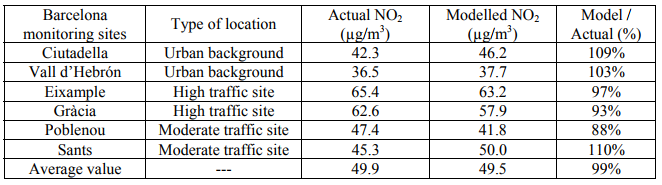
\includegraphics[scale=1.4]{de_nazelle_model_performance}
\caption{Performance statistics of an air quality model used in \cite{DeNazelle2013}}
\label{tab:fig:de_nazelle_model_performance}
\end{figure}

By understanding the scale of these errors in the air quality model, if it is presumed that they are uniform in time and space across the study area (discussed more below), then they can be incorporated into a static exposure study of outdoor air at household addresses or similar.

%%%%%%%%%%%%%%%%%%%%%%%%%%%%%%
\subsection{Air quality annual average non-monitoring site predictions}
\label{air_quality_annual_average_non_site_predictions}
%%%%%%%%%%%%%%%%%%%%%%%%%%%%%%

The predictions of air quality models, away from monitoring sites, is less well understood. Taking our 2016 CMAQ-UK model the NO$_{2}$ map of London shown in Figure \ref{fig:cmaq_and_monitoring_sites} (below) illustrates the location of monitoring sites i.e. where the predictions have been evaluated and understood. Clearly there are many areas which are not evaluated; there are 16 million cells in the raster, and only 242 sites (many of which are either not operational, do not have a high enough data capture rate for comparison, or do not measure the pollutants we are interested in, meaning the actual number is far less). This means that only ~0.0015\% of the locations shown in Figure \ref{fig:cmaq_and_monitoring_sites} have been evaluated and the possible error (between model prediction and measurement) understood.

\begin{figure}[H]
\centering
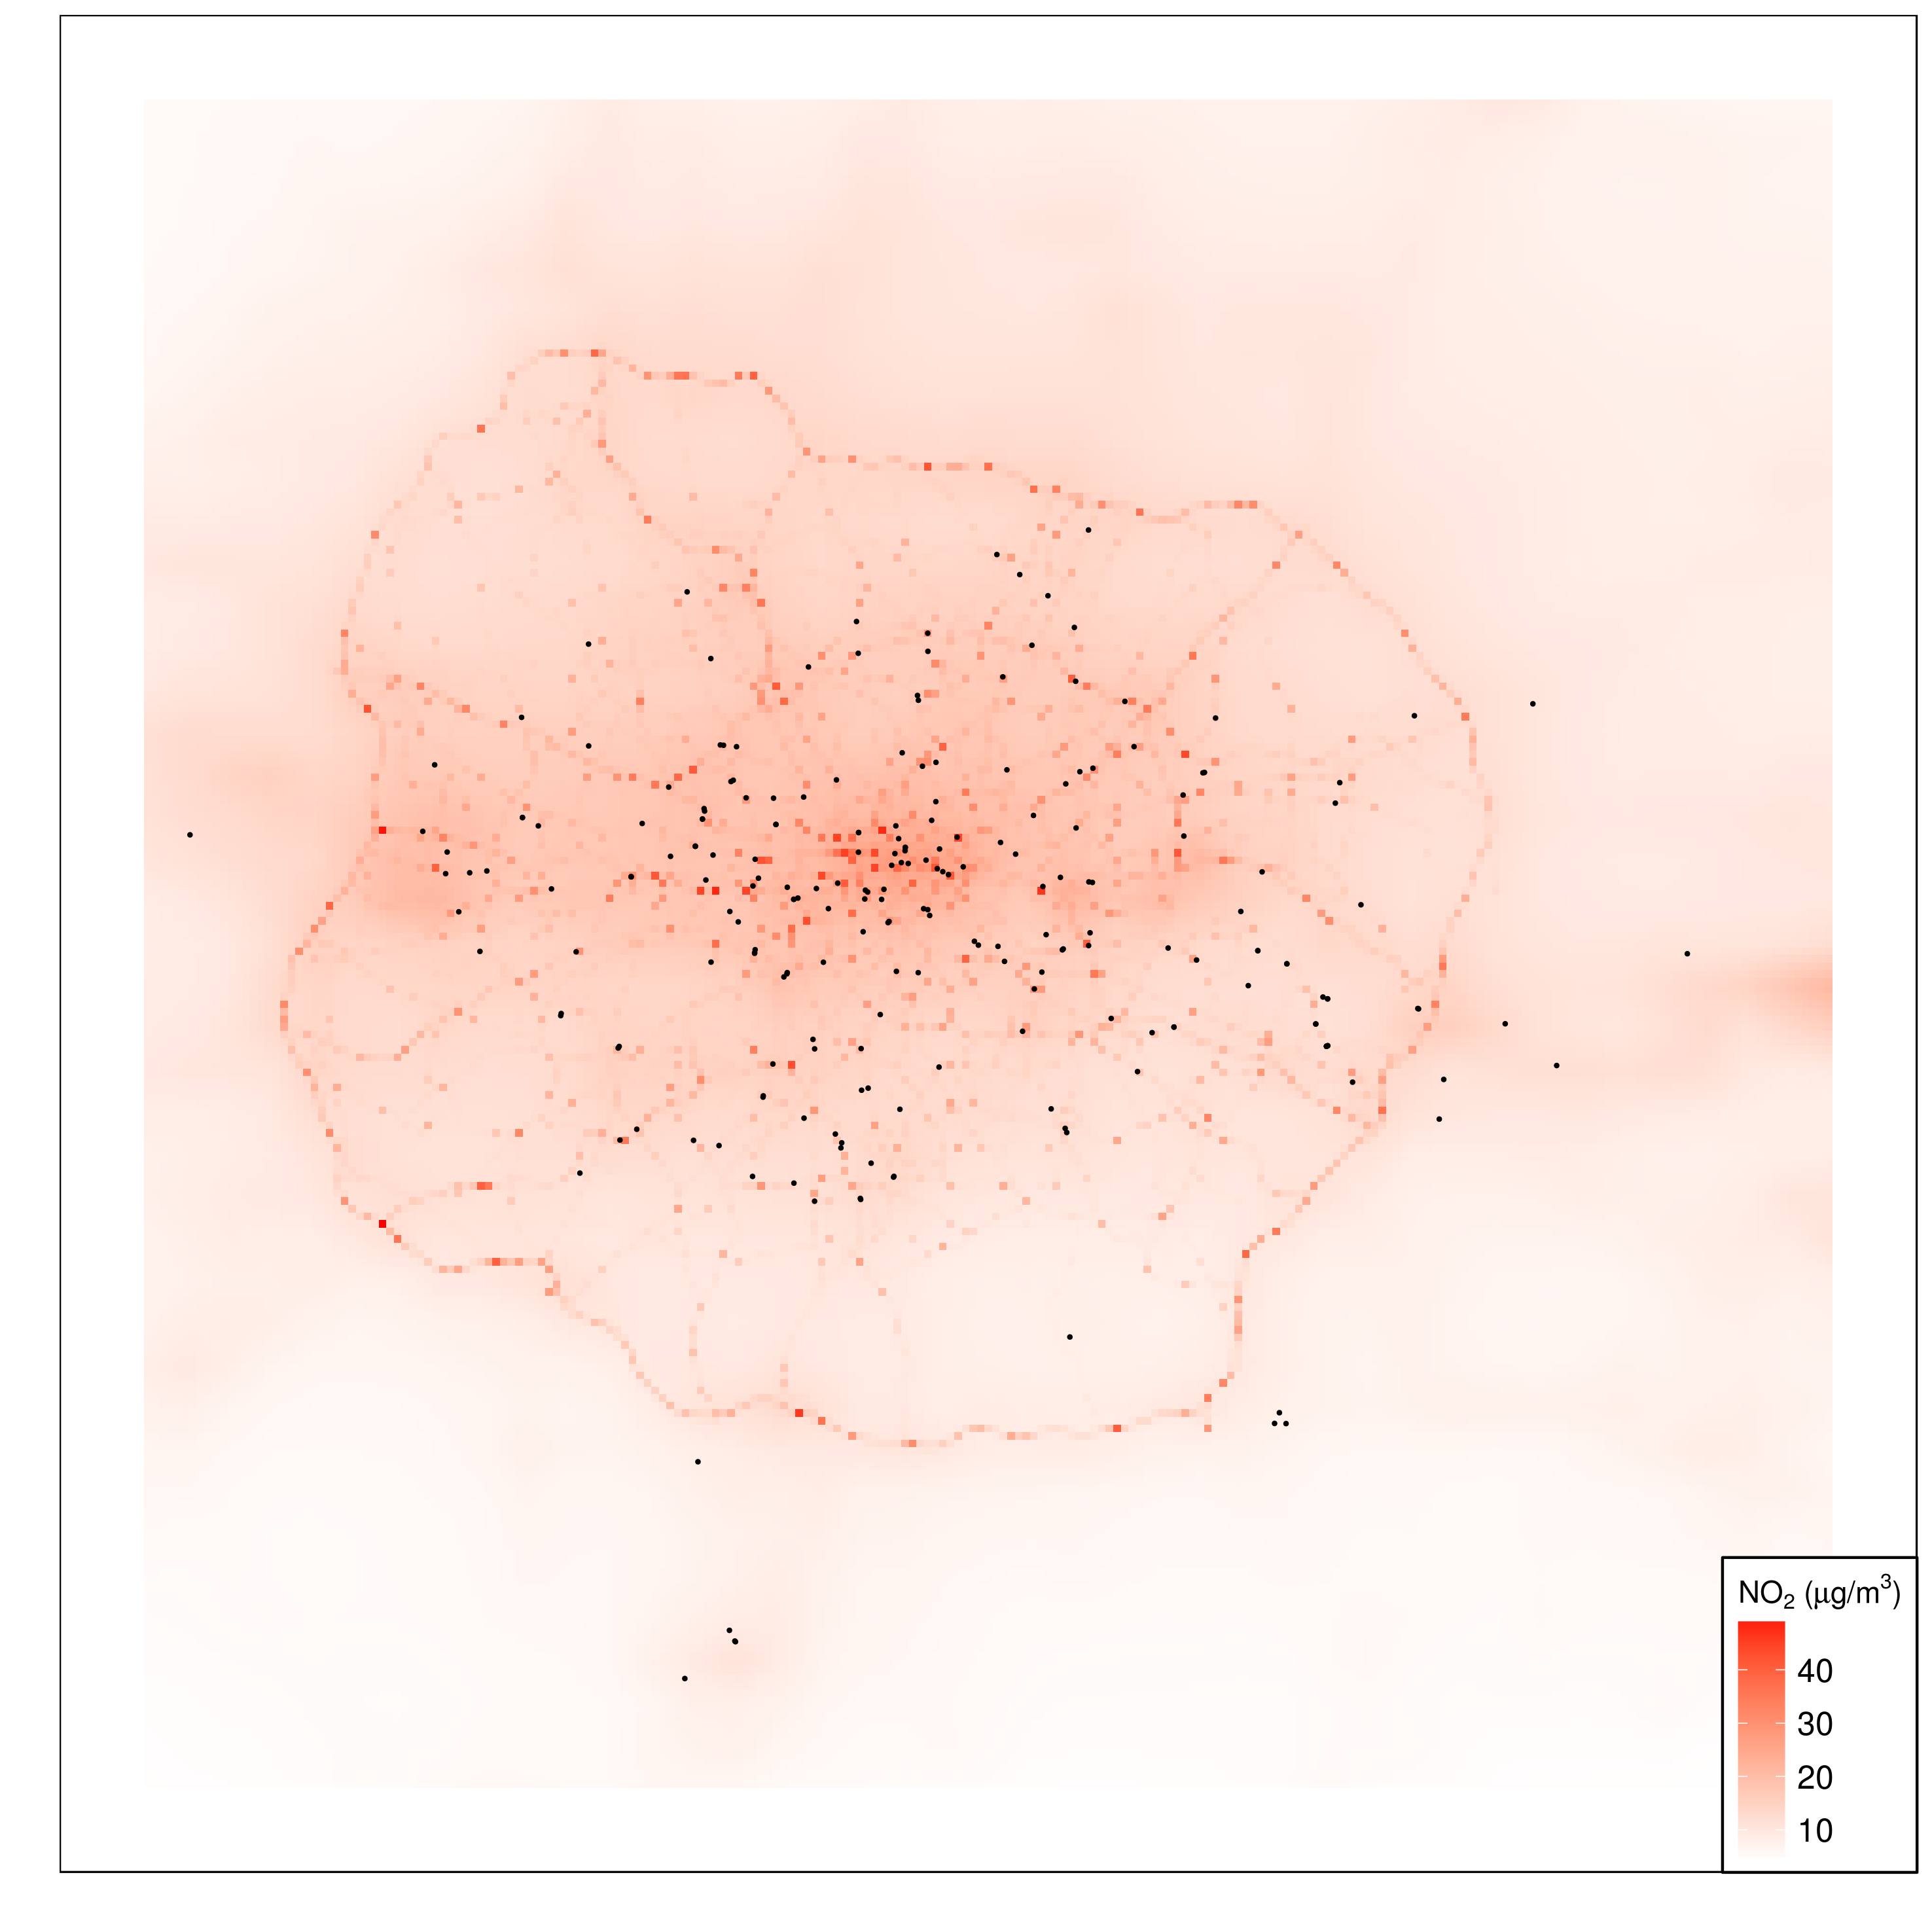
\includegraphics[scale=0.5]{images/cmaq_and_monitoring_sites.png}
\caption{CMAQ-UK for London + Air Quality monitoring sites}
\label{fig:cmaq_and_monitoring_sites}
\end{figure}

For these non-monitoring site locations, we presume that the model functions in the same manner, with the same error levels. In reality it seems likely that there are varying degrees of accuracy. This may be less of a concern within an exposure model looking at health effects between areas of high/low concentrations, providing it represents the spatial pattern adequately i.e. predicting lower concentrations and higher concentrations in the right places, even if the concentrations themselves are not exactly right. As part of this chapter I am going to aim to better understand how the model predicts away from monitoring sites. It is impractical to place a monitoring site at every location, so I will develop a method whereby I use mobile monitoring devices in-lieu of monitoring sites. As background to this, I searched for studies which have already attempted this. There is a small amount of literature which has tried to evaluate air quality away from monitoring sites using mobile monitors. \cite{Buteau2017} compared a number of methods for predicting concentrations of O3 and NO$_{2}$ in Montreal, Canada at the level three-character postal code area (~6km$^{2}$ square). Alongside traditional spatial interpolation using inverse-distance weighting, and nearest monitoring site methods, they also based a land-use regression model upon a dense monitoring survey. However, these were semi-permanent monitors at fixed sites for 9 months of a year, and so whilst their results were encouraging the method is not really transferable to portable monitors that I intend to use. \cite{Shi2016} also created a land-use regression model, with mobile measurements as an input, which achieved good results, but their study was based on repeated measurements using vehicles sampling along a set route for 14 consecutive days, and the choice of 14 rather than say 20 seemed to be a function of their available sampling time rather than calculated using statistical analysis.

%%%%%%%%%%%%%%%%%%%%%%%%%%%%%%
\subsection{Air quality temporal predictions}
\label{air_quality_temporal_predictions}
%%%%%%%%%%%%%%%%%%%%%%%%%%%%%%

Air quality models that use a higher temporal resolution have more sources of error to quantify and include in an exposure model than one which uses annual averages. As an annual average value, a difference of +/- 5 $\mu \text{g m}^{-3}$ between the model and the measurements can be factored into the exposure prediction relatively easily. But if the model is predicting a concentration every hour then this error will vary for each hour i.e. 8760 hours resulting in 8760 model/measurement differences.

%%%%%%%%%%%%%%%%%%%%%%%%%%%%%%
\subsection{Micro-environmental modelling}
\label{microenvironmental_modelling}
%%%%%%%%%%%%%%%%%%%%%%%%%%%%%%

Within dynamic exposure models, exposure in microenvironments is often calculated in relation to outdoor concentrations. Therefore, in addition to the uncertainty of the air quality predictions in a place and time, further uncertainty is added when the outdoor concentration is ‘converted’ to a microenvironment concentration (whether this is done using an I/O ratio for indoor concentrations, or a mass-balance model as used in Section \ref{sec:in_vehicle_modelling}). Exposures in the LHEM, for all environments except the London Underground, used the CMAQ-UK air quality model as an input. \cite{Dhondt2012} described the possible sources of error within the in-vehicle section of their dynamic model, and noted that the air quality inputs may not be of a high enough spatial resolution to capture concentration gradients near roads adequately. But they did not seek to evaluate the individual-level daily/weekly/hourly concentrations, and indeed due to the type of the study (an aggregated population) they would have found it difficult to do so (due to the large numbers of individuals). Similarly and whilst this was evaluated at monitoring sites (Figure \ref{tab:fig:de_nazelle_model_performance}), no monitoring attempt at individual level exposure evaluation was undertaken.

%%%%%%%%%%%%%%%%%%%%%%%%%%%%%%
\subsection{Representative errors}
\label{representative_errors}
%%%%%%%%%%%%%%%%%%%%%%%%%%%%%%

Exposure predictions for an individual or group, over a time period, can be made using dynamic models. But the degree to which these predictions are representative of that exposure for that period of time is a source of uncertainty. Similarly, the degree to which predicting exposure for a group or groups of people, and extrapolating to the wider population, is a further source of confusion and error. In the LHEM, the exposures for each individual were calculated based on the person’s previous days’ movements, and they were asked whether this was representative of their typical day. Analysing the responses to the latter question showed us that most of the subjects had a fairly set pattern of movement (and therefore likely exposure), but the degree of the variance between their typical day and a non-typical day is unknown, and indeed how many ‘non-typical days’ do they have? One way to evaluate the exposure predictions from our model would have been to distribute personal monitors to all the LTDS participants, for an entire year, collect and process the data, and then compare it to the LHEM predictions to see whether our ‘snap shot’ day exposure was close to their annual average day exposure. However, there were ~45,000 subjects, meaning a huge number of personal monitors and logistical support would have been needed, and it was therefore unfeasible. A method to make this more manageable might be to develop a statistical model whereby an appropriate sample-size is calculated. That is, just sampling a percentage of the 45,000, but in the knowledge that they will have a similar distribution of exposures to the total population of the study; then giving this smaller subset of participants monitors for a prolonged period of time and understanding the daily changes in their exposure. This is explored more in Methods (Section \ref{sec:4methods}) 

%%%%%%%%%%%%%%%%%%%%%%%%%%%%%%%%%%%%%%%%%%%%%%%%%%%%%%%%%%%%%%%%%%%%%%%%%%%%%%%%%%%
\section{Methods}
\label{sec:4methods}
%%%%%%%%%%%%%%%%%%%%%%%%%%%%%%%%%%%%%%%%%%%%%%%%%%%%%%%%%%%%%%%%%%%%%%%%%%%%%%%%%%%

We can now see that there are a number of difficult and challenging sources of error to consider in evaluating a hybrid exposure model. Air quality models have quantifiable errors in their predictions at the monitoring sites they are evaluated against, errors at locations away from monitoring sites which are not well understood, further variation and errors when using a high time resolution air quality model, errors in the micro-environmental modelling, and more errors in terms of the representativeness of the exposure predictions arrived at. The following methods section outlines how I attempt to mitigate some of these sources of error, remove some of the others, and produce an evaluation of one short journey; comparing the LHEM prediction of this journey to measured exposure using personal monitoring. The process is summarised below in Figure \ref{fig:comparison_method_summary}.

\begin{figure}[H]
\centering
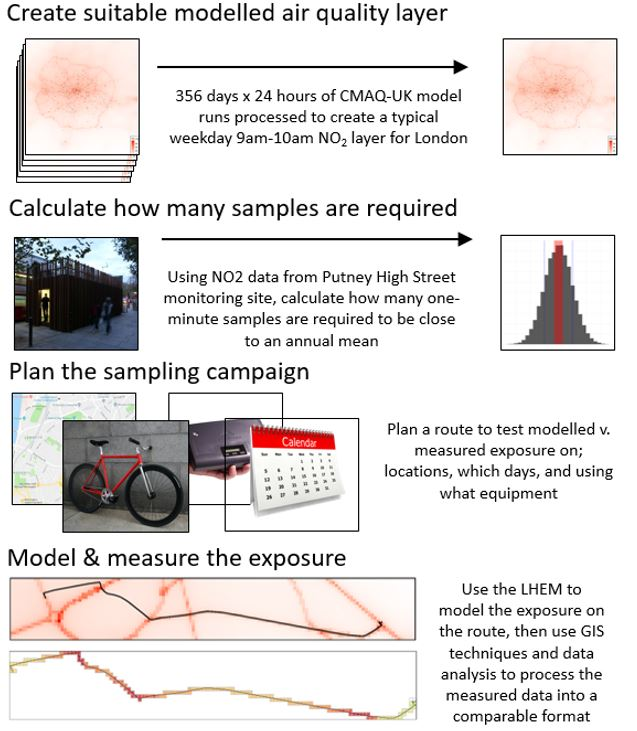
\includegraphics[scale=0.8]{images/comparison_method_summary.jpg}
\caption{Method summary}
\label{fig:comparison_method_summary}
\end{figure}

%%%%%%%%%%%%%%%%%%%%%%%%%%%%%%
\subsection{Modelled Air Quality}
\label{subsec:4modelledairquality}
%%%%%%%%%%%%%%%%%%%%%%%%%%%%%%

The exposures in the LHEM contained Londoners movement data covering twelve months of the year between 2005 and 2011. The CMAQ-UK air quality model used was an annual average hourly weekday/Saturday/Sunday model of 2011 air quality, and linked to the movement of the individual based on what day of the week their time-activity data was recorded. The air quality model for this chapter is a 2016 CMAQ-UK output, with appropriate emissions and meteorology, cropped to London, but otherwise unchanged in methods from the 2011 model. When evaluated on an annual average basis i.e. one value for each 20m x 20m grid square of London, this new 2016 model performs well (Table \ref{tab:cmaq_performance_stats_2016}).


\begin{table}[H]
\scriptsize
\centering
\begin{tabular}{|p{1cm}|p{1cm}|p{0.8cm}|p{1cm}|p{0.6cm}|p{1cm}|p{1cm}|p{0.8cm}|p{0.8cm}|p{0.8cm}|p{0.6cm}|p{0.7cm}|}
\hline
\textbf{Pollutant} & \textbf{Number of data} & \textbf{Mean obs} & \textbf{Mean Mod} & \textbf{FAC2} & \textbf{MB} & \textbf{MGE} & \textbf{NMB} & \textbf{NMGE} & \textbf{RMSE} & \textbf{r} & \textbf{COE} \\ \hline
CO         & 2  & 369.79 & 318.75 & 1    & -51.04 & 72.08 & -0.14 & 0.19 & 88.32 & 1    & 0.50  \\ \hline
NO$_{2}$   & 73 & 51.80  & 48.49  & 1    & -3.30  & 9.01  & -0.06 & 0.17 & 13.79 & 0.84 & 0.52  \\ \hline
NO$_{x}$   & 72 & 134.74 & 108.52 & 0.97 & -26.23 & 39.52 & -0.19 & 0.29 & 61.50 & 0.78 & 0.43  \\ \hline
O$_{3}$    & 16 & 29.74  & 35.40  & 1    & 5.66   & 6.59  & 0.19  & 0.22 & 7.81  & 0.83 & 0.07  \\ \hline
PM$_{10}$  & 56 & 22.76  & 22.74  & 1    & -0.03  & 2.93  & 0.00  & 0.13 & 4.14  & 0.57 & 0.22  \\ \hline
PM$_{2.5}$ & 23 & 13.08  & 12.34  & 1    & -0.74  & 1.85  & -0.06 & 0.14 & 2.30  & 0.72 & 0.20  \\ \hline
\end{tabular}
\caption{Annual average performance statistics for CMAQ-UK 2016}
\label{tab:cmaq_performance_stats_2016}
\end{table}

We can see that the RMSE values for the pollutants range from 88.32 PPB for CO down to 2.3 $\mu \text{g m}^{-3}$ for PM$_{10}$. For NO$_{2}$, which is the pollutant being focused on in this chapter, the RMSE is 13.79 $\mu \text{g m}^{-3}$. An exposure model using annual average NO$_{2}$ predictions from this 2016 CMAQ-UK air quality model could incorporate these errors; a prediction of 40 $\mu \text{g m}^{-3}$, presuming a normal distribution of errors, would therefore actually be anywhere within the range of 26.21 $\mu \text{g m}^{-3}$ to 53.79 $\mu \text{g m}^{-3}$. The exposure-health relationships investigated by epidemiologists could then take this into account. Moving to a higher temporal scale, the daily-hourly version of this same model (Table \ref{tab:cmaq_performance_stats_2016_hourly}) performs less well for NO$_{2}$ than the annual average shown above (Table \ref{tab:cmaq_performance_stats_2016}).

\begin{table}[H]
\scriptsize
\centering
\begin{tabular}{|p{1cm}|p{1cm}|p{0.8cm}|p{1cm}|p{0.6cm}|p{1cm}|p{1cm}|p{0.8cm}|p{0.8cm}|p{0.8cm}|p{0.6cm}|p{0.7cm}|}
\hline
\textbf{Pollutant} & \textbf{Number of data} & \textbf{Mean obs} & \textbf{Mean Mod} & \textbf{FAC2} & \textbf{MB} & \textbf{MGE} & \textbf{NMB} & \textbf{NMGE} & \textbf{RMSE} & \textbf{r} & \textbf{COE} \\ \hline
CO         & 24520  & 408.92 & 338.26 & 0.78 & -70.65 & 175.22 & -0.17  & 0.43 & 259.18 & 0.53 & 0.23  \\ \hline
NO$_{2}$   & 656419 & 52.10  & 49.01  & 0.84 & -3.09  & 18.63  & -0.06  & 0.36 & 28.32  & 0.69 & 0.35  \\ \hline
NO$_{x}$   & 649220 & 136.27 & 110.28 & 0.68 & -25.99 & 70.72  & -0.19  & 0.52 & 129.38 & 0.63 & 0.36   \\ \hline
O$_{3}$    & 148043 & 28.84  & 34.31  & 0.66 & 5.46   & 12.88  &  0.19  & 0.45 & 17.20  & 0.74 & 0.30   \\ \hline
PM$_{10}$  & 49461  & 22.96  & 22.87  & 0.89 & -0.09  & 7.07   &  0.00  & 0.31 & 11.89  & 0.70 & 0.35   \\ \hline
PM$_{2.5}$ & 188237 & 13.15  & 12.44  & 0.85 & -0.71  & 3.72   &  -0.05 & 0.28 & 5.76   & 0.86 & 0.51  \\ \hline
\end{tabular}
\caption{Daily-hourly performance statistics for CMAQ-UK 2016}
\label{tab:cmaq_performance_stats_2016_hourly}
\end{table}

The NO$_{2}$ predictions have an R value down from 0.84 to 0.68 and a RMSE up from 13 $\mu \text{g m}^{-3}$ to 28.32. Using a higher temporal scale model has increased the uncertainty of the air quality concentration predictions to the model.

To evaluate the LHEM using this air quality as an input, we needed to decide what time period of exposure to try and replicate with measurements. Evaluating at a higher time resolution than annual average was preferable, but a very high time resolution would be difficult as this would mean needing to take a huge number of measurements. For example supposing we wanted to evaluate exposure on Saturday’s between 11am and 2pm and how the LHEM modelled this (within the context of a journey); measurements would need to be taken continuously on the journey in question every Saturday throughout the year between 11am and 2pm to compare the measurements with the modelled air quality output (putting the spatial and micro-environmental factors aside for a moment). 
To simplify the evaluation, and make the experiment a reasonable undertaking, the timeframe that it would be performed over was restricted, so rather than cover a whole year we considered August and September only, on weekdays, and between the hours of 9am of 10am. To create an appropriate air quality model for this time period, 365 days of CMAQ-UK layers were used (each with 24 hours). A loop was written in R to download the raw CMAQ-UK NetCDF model files, convert them to standard raster R files, combine the individual files for each hour of the two months in question, discard data that was not 9am to 10am, and then take the mean for each grid square. The concentrations were outputted in PPB, so were converted to $\mu \text{g m}^{-3}$ using the EU standard of 1.9125. Figure 3 shows the result of this process i.e. the models predicted air quality for a typical weekday in August or September between 9am and 10am.

\begin{figure}[H]
\centering
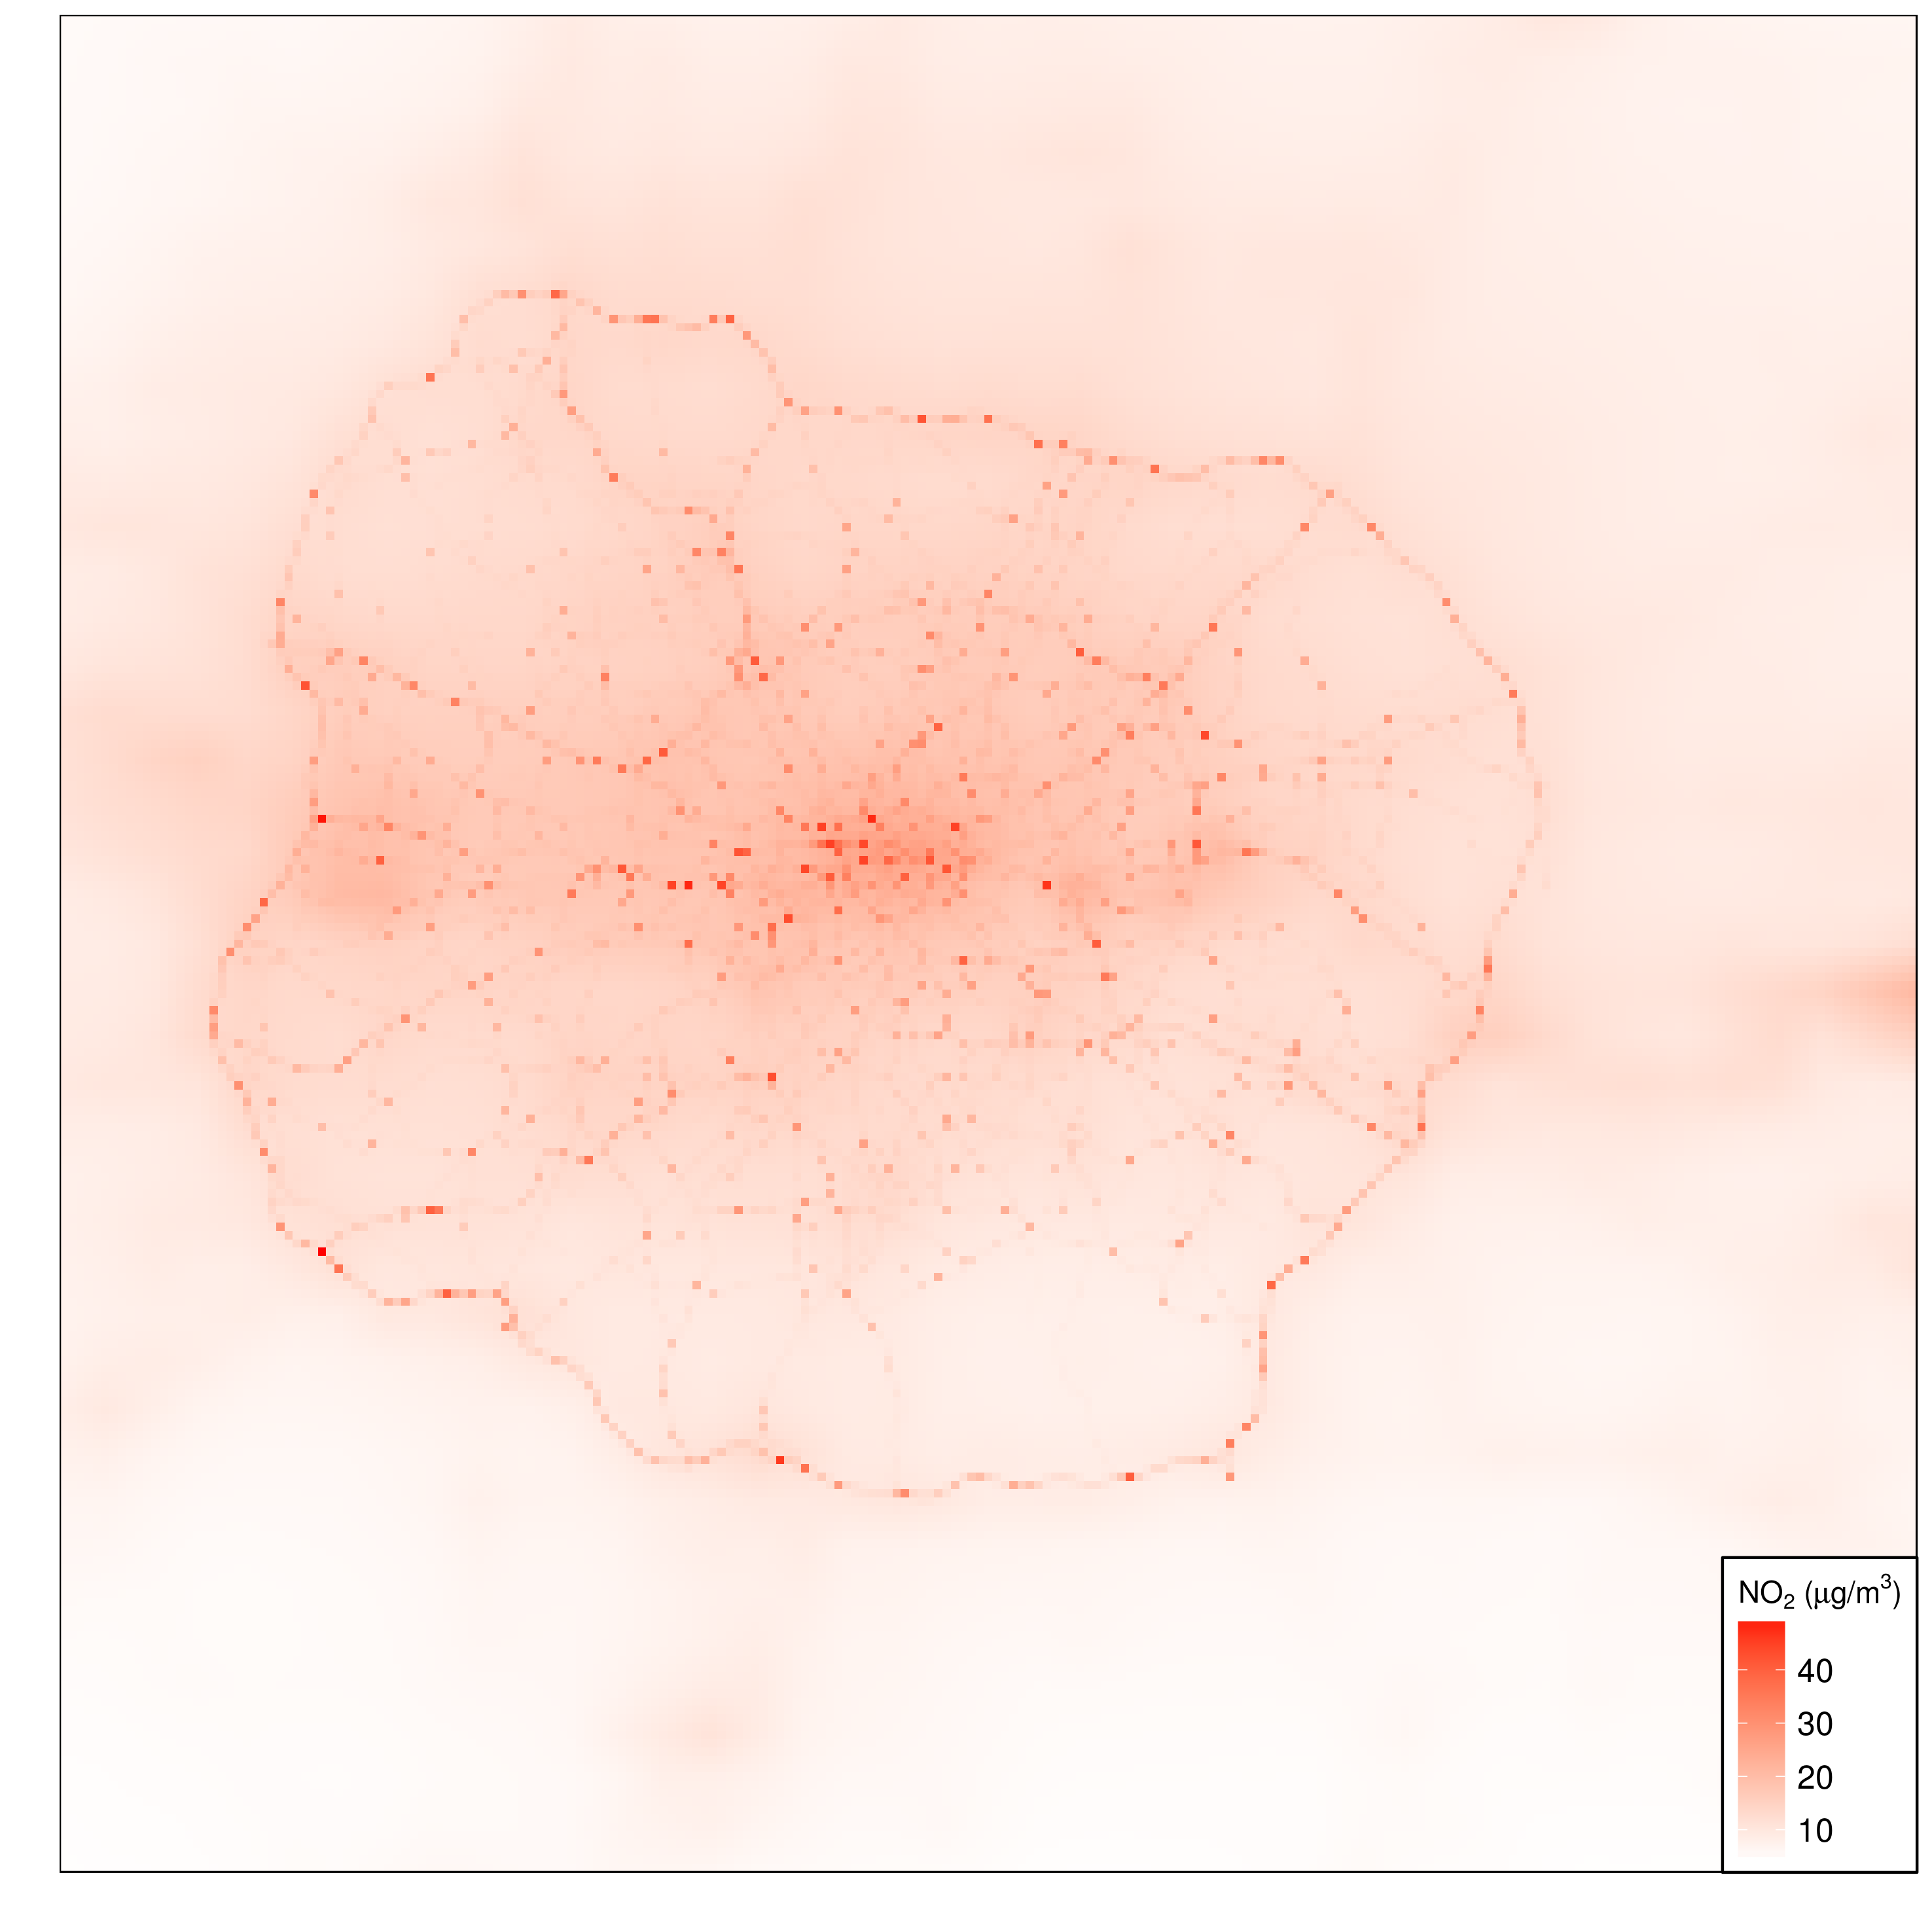
\includegraphics[scale=0.4]{cmaq_aug_sept.png}
\caption{CMAQ-UK air quality model for 9am to 10am on weekdays in August/September}
\label{fig:cmaq_aug_sept}
\end{figure}

%%%%%%%%%%%%%%%%%%%%%%%%%%%%%%
\subsection{Micro-environmental adjustments}
\label{subsec:4microenvironmentaladjustments}
%%%%%%%%%%%%%%%%%%%%%%%%%%%%%%

As discussed in the introduction to this chapter, and within  Section \ref{subsec:microenvironments}, calculating exposure within micro-environments in relation to outdoor concentrations is not a well understood area of science and seems to be susceptible to a great deal of variation depending on conditions of the micro-environment (and other factors). To simplify, I decided to effectively remove this uncertainty from my evaluation by considering the exposure of a journey which did not need micro-environmental modelling, looking at journeys of the LHEM that take concentrations directly from CMAQ-UK i.e. walking and cycling. This is not to say that this is an unimportant area for investigation, due to the large amount of time that people spend indoors it clearly is, but I need to compartmentalise this chapter in order to make the research achievable, and this is an area that can be reasonably removed.

%%%%%%%%%%%%%%%%%%%%%%%%%%%%%%
\subsection{Sample size}
\label{subsec:samplesize}
%%%%%%%%%%%%%%%%%%%%%%%%%%%%%%

Having established that I will look to evaluate exposure on a cycling journey between 9am and 10am on weekdays in August and September, I now needed to establish how many cycling journeys (and measurements) would be needed to represent modelled exposure of this same journey. Repeat measurements will be needed as although CMAQ-UK has well resolved temporal and spatial inputs such as vehicle numbers and emissions by time of day and day of the week, with similar meteorological inputs, it cannot take account of inter-day variability of an unpredictable nature e.g. a car breaking down leading to a traffic jam, and increased emissions for an hour of a Saturday morning. By taking repeat measurements, the effects of these type of events on the evaluation should be reduced. But exactly how many we are not sure. 
We can consider this question in a theoretical framework to start-with, based around the LHEM. If we presume that the mean daily PM2.5 exposures of the 45,000 LTDS subjects was 15 ug/m3, with a standard deviation of 2.5 ug/m3, and we use a random number generator with these parameters to assign each subject an exposure, we end up with a distribution like Figure \ref{fig:theoretical_lhem_pm25}.

\begin{figure}[H]
\centering
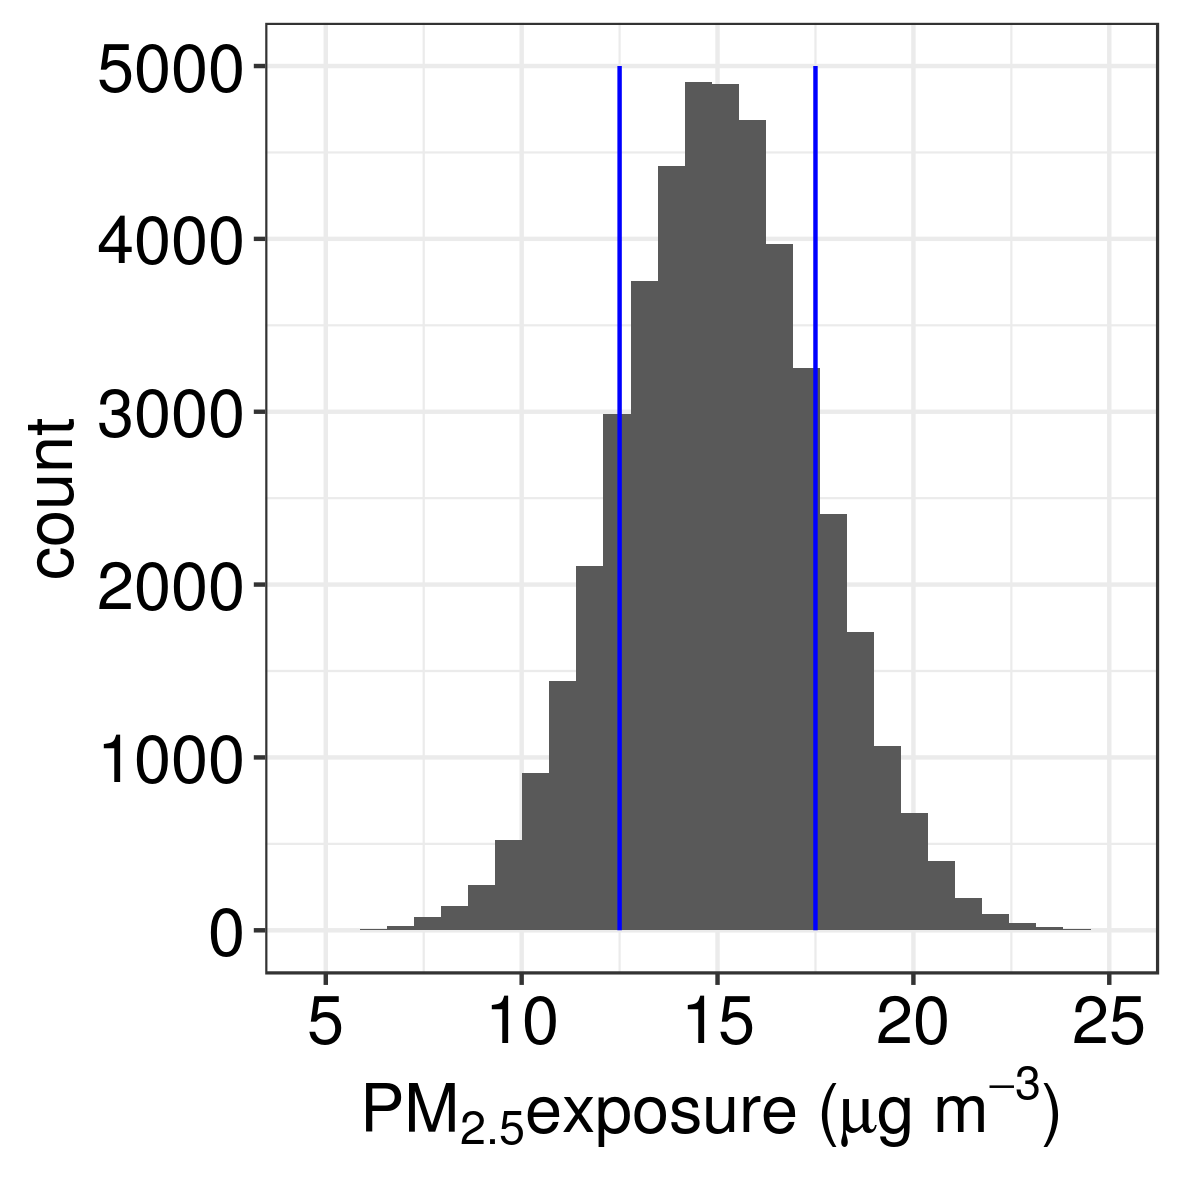
\includegraphics[scale=1]{theoretical_lhem_pm25.png}
\caption{Theoretical LHEM exposures of 45,000 subjects based on a pre-defined mean of 15 $\mu \text{g m}^{-3}$ and a standard deviation of 2.5 $\mu \text{g m}^{-3}$ (shown in blue)}
\label{fig:theoretical_lhem_pm25}
\end{figure}

This distribution of these exposures has a mean of 15 $\mu \text{g m}^{-3}$, a standard deviation of 2.5 $\mu \text{g m}^{-3}$, a max of 25.19 $\mu \text{g m}^{-3}$ and a min of 5.61 $\mu \text{g m}^{-3}$. If these were the real exposures of the LHEM subjects, and we wanted to undertake measurements on a sub-sample to evaluate our model, and we decided we would be happy with our sub-sample having a mean within 10\% of the population mean (15 $\mu \text{g m}^{-3}$), with 95\% confidence, we can then solve a sample size calculation (REF) and arrive at the answer of 43. That is, we only need to sample 43 people to evaluate the model within these parameters.  However this is just going to give us a sample distribution, that we can be relatively certain has a mean that is within the area highlighted in red in Figure \ref{fig:theoretical_lhem_pm25_samples}, but may or may not have the same shape of distribution, maximum, minimum, standard deviation etc. of the population. We are also likely to miss evaluating the exposures of the subjects who have exposures in the highest and lowest percentiles of the data, which as discussed in Section \ref{subsec:longtermvshortterm} may be important for understanding health effects.

\begin{figure}[H]
\centering
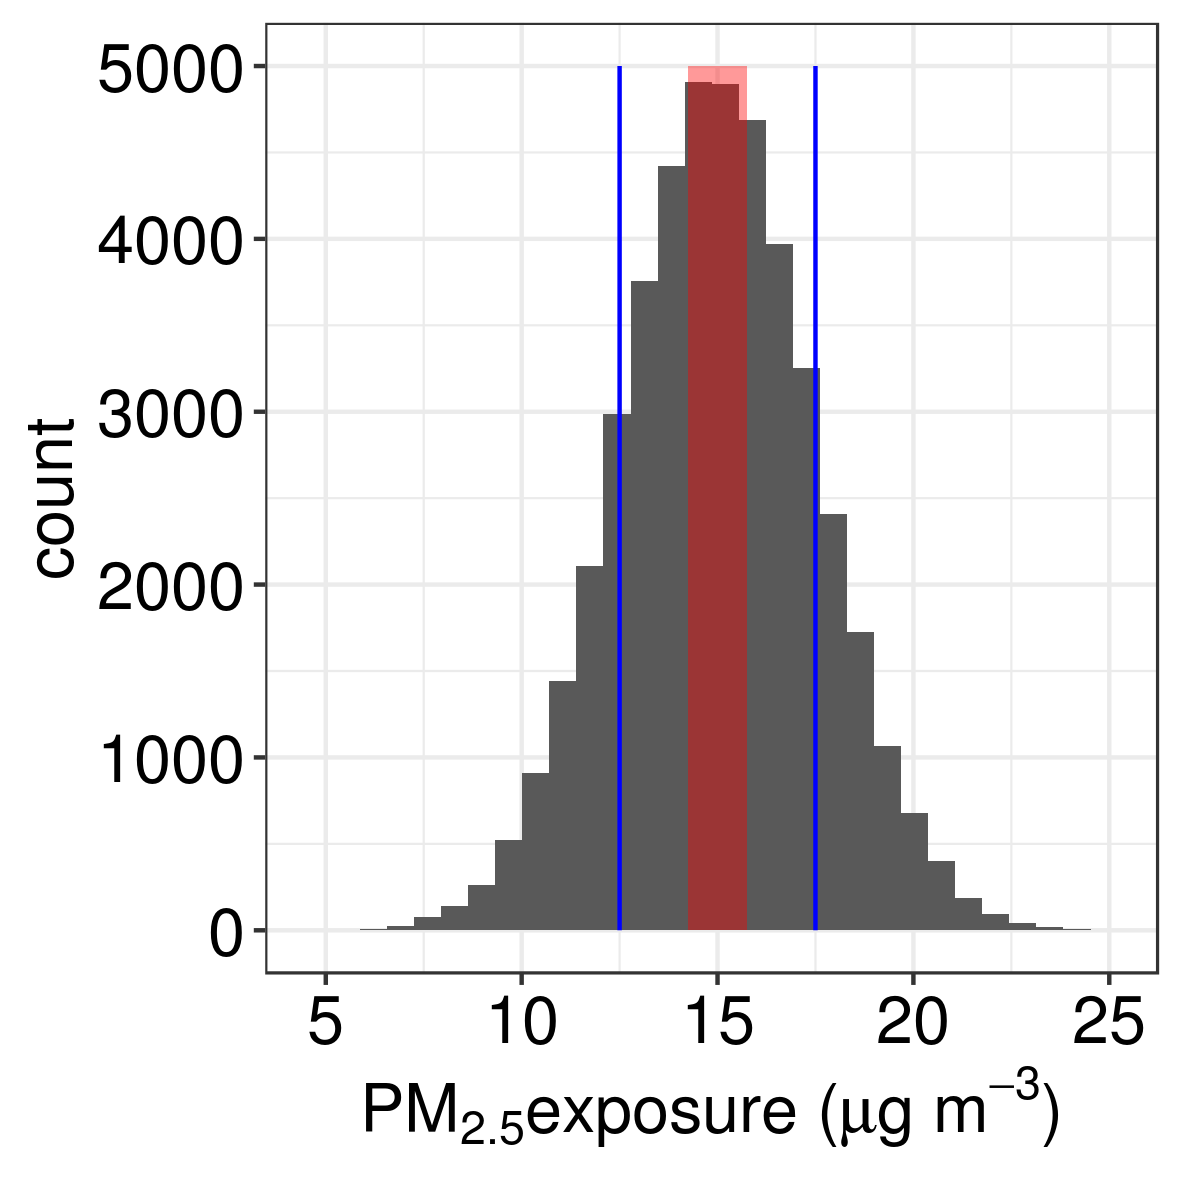
\includegraphics[scale=1]{theoretical_lhem_pm25_samples.png}
\caption{Theoretical LHEM exposures of 45,000 subjects based on a pre-defined mean of 15 $\mu \text{g m}^{-3}$ and a standard deviation of 2.5 $\mu \text{g m}^{-3}$ (shown in blue), with the mean of a sub-sample of 43 subjects (within the red area)}
\label{fig:theoretical_lhem_pm25_samples}
\end{figure}

To properly capture the distribution of the population in a sample we need to do stratified random sampling, ensuring proportional representation of each strata (exposure concentrations in our case).  However, to do this we would already need to have a priori understanding of the exposures of the larger group, and the drivers of the exposures, in order to be able to calculate the numbers of samples required from each strata.
Given the difficultly in trying to evaluate a typical day of an individual in the LHEM and how these fit against an annual average, I will again simplify. By just evaluating the modelled and measured exposure of a single cycling journey from the LHEM most of these issues are put aside. I just need to calculate how many measurements of the journey on a weekday between 9am and 10am in August and September are needed to represent (within predefined boundaries) the typical exposure on the journey to compare to the model.
I calculated this using one-minute data from a monitoring site (as a known, continuous, and reliable dataset), and then running sample size calculations on it, as a proxy for a CMAQ-UK grid square in the model. I took one year of one minute NO2 monitoring data from the site ‘Wandsworth - Putney High Street’, removed the data outside of our time period of interest (weekdays, 9am to 10am in August and September), and then calculated summary statistics on the remaining data (Shown in Table \ref{tab:wa7_summary_stats}). I chose this monitoring site as the site collects one-minute resolution NO$_{2}$ data, which aligns with the temporal resolution of the equipment I intend to use for monitoring.

\begin{table}[H]
\centering
    \begin{tabular}{ | l | l |}
    \hline 
     \bfseries{Statistic}   & \bfseries{NO$_{2}$ $\mu \text{g m}^{-3}$}    \\ \hline
     Minutes                & 2400                                         \\ \hline
     Mean                   & 90.92                                        \\ \hline
     Median                 & 77.70                                        \\ \hline
     Max                    & 1074.4                                       \\ \hline
     Min                    & 11.67                                        \\ \hline
     Standard deviation     & 64.23                                        \\ \hline
    \end{tabular}
\caption{Site WA7 summary statistics for weekday, 9am-10am during}
\label{tab:wa7_summary_stats}
\end{table}

Now that I had summary statistics for the period of time of interest, I calculated how many samples were required within this time period to create a similar distribution and mean, as per the theoretical example from Figures \ref{fig:theoretical_lhem_pm25} and \ref{fig:theoretical_lhem_pm25_samples} using Equation \ref{eq:sample_size_equation_pt1} (\cite{PennStateEberlyCollegeofScience2017}). By taking this reliable and continuous dataset, in a known location, we extrapolate the results to locations where there is not a fixed site data collection method available.

\begin{equation}
  \chi = \textit{Z}^2 \times \frac{\sigma^2}{moe^2} 
  \label{eq:sample_size_equation_pt1}
\end{equation}

Where $\chi$ is the calculated sample size, \textit{Z} is the z-score of the desired confidence level, $\sigma$ is the standard deviation of the population (concentrations), and \textit{moe} is the allowed margin of error (in $\mu \text{g m}^{-3}$). By writing a loop in the R programming language (\cite{RFoundationforStatisticalComputing2014}), and testing a variety of input variables to this equation, I was able to see how many samples would be required in different scenarios of confidence levels and allowable margins of error. The results are shown in Table \ref{tab:no2_samples_needed}:

\begin{table}[H]
\centering
\begin{tabular}{|l|l|l|}
\hline
Confidence level     &            Allowed margin of error                            &        Sample required       \\ hline
\multirow{6}{*}{99\%}   &            10\% ($\pm$ 9   $\mu \text{g m}^{-3}$ )    &        1325                  \\ \cline{2-3} 
                        &            15\% ($\pm$ 14  $\mu \text{g m}^{-3}$ )    &        589                   \\ \cline{2-3} 
                        &            20\% ($\pm$ 18  $\mu \text{g m}^{-3}$ )    &        331                   \\ \cline{2-3}
                        &            25\% ($\pm$ 23  $\mu \text{g m}^{-3}$ )    &        212                   \\ \cline{2-3}
                        &            30\% ($\pm$ 27  $\mu \text{g m}^{-3}$ )    &        147                   \\ \cline{2-3}
                        &            35\% ($\pm$ 32  $\mu \text{g m}^{-3}$ )    &        108                   \\ \hline
\multirow{6}{*}{95\%}   &            10\% ($\pm$ 9   $\mu \text{g m}^{-3}$ )    &        767                   \\ \cline{2-3} 
                        &            15\% ($\pm$ 14  $\mu \text{g m}^{-3}$ )    &        341                   \\ \cline{2-3} 
                        &            20\% ($\pm$ 18  $\mu \text{g m}^{-3}$ )    &        192                   \\ \cline{2-3} 
                        &            25\% ($\pm$ 23  $\mu \text{g m}^{-3}$ )    &        123                   \\ \cline{2-3} 
                        &            30\% ($\pm$ 27  $\mu \text{g m}^{-3}$ )    &        85                    \\ \cline{2-3} 
                        &            35\% ($\pm$ 32  $\mu \text{g m}^{-3}$ )    &        63                    \\ \hline
\multirow{6}{*}{90\%}   &            10\% ($\pm$ 9   $\mu \text{g m}^{-3}$ )    &        540                   \\ \cline{2-3} 
                        &            15\% ($\pm$ 14  $\mu \text{g m}^{-3}$ )    &        240                   \\ \cline{2-3} 
                        &            20\% ($\pm$ 18  $\mu \text{g m}^{-3}$ )    &        135                   \\ \cline{2-3} 
                        &            25\% ($\pm$ 23  $\mu \text{g m}^{-3}$ )    &        86                    \\ \cline{2-3} 
                        &            30\% ($\pm$ 27  $\mu \text{g m}^{-3}$ )    &        60                    \\ \cline{2-3} 
                        &            35\% ($\pm$ 32  $\mu \text{g m}^{-3}$ )    &        44                    \\ \hline
\multirow{6}{*}{85\%}   &            10\% ($\pm$ 9   $\mu \text{g m}^{-3}$ )    &        414                   \\ \cline{2-3} 
                        &            15\% ($\pm$ 14  $\mu \text{g m}^{-3}$ )    &        184                   \\ \cline{2-3} 
                        &            20 \% ($\pm$ 18 $\mu \text{g m}^{-3}$ )    &        103                   \\ \cline{2-3} 
                        &            25\% ($\pm$ 23  $\mu \text{g m}^{-3}$ )    &        66                    \\ \cline{2-3} 
                        &            30\% ($\pm$ 27  $\mu \text{g m}^{-3}$ )    &        46                    \\ \cline{2-3} 
                        &            35\% ($\pm$ 32  $\mu \text{g m}^{-3}$ )    &        34                    \\ \hline
\multirow{6}{*}{80\%}   &            10\% ($\pm$ 9   $\mu \text{g m}^{-3}$ )    &        327                   \\ \cline{2-3} 
                        &            15\% ($\pm$ 14  $\mu \text{g m}^{-3}$ )    &        145                   \\ \cline{2-3} 
                        &            20\% ($\pm$ 18  $\mu \text{g m}^{-3}$ )    &        82                    \\ \cline{2-3} 
                        &            25\% ($\pm$ 23  $\mu \text{g m}^{-3}$ )    &        52                    \\ \cline{2-3} 
                        &            30\% ($\pm$ 27  $\mu \text{g m}^{-3}$ )    &        36                    \\ \cline{2-3} 
                        &            35\% ($\pm$ 32   $\mu \text{g m}^{-3}$ )   &        27                    \\ \hline
\end{tabular}
\caption{Numbers of samples required for each confidence level and allowable margin of error based on measurements from WA7}
\label{tab:no2_samples_needed}
\end{table}

From these calculations we can see that to get a result which is within 10 $\mu \text{g m}^{-3}$ of the mean, with 99\% confidence, 1325 samples would need to be taken, at random in the time window, in a grid square. Given my aim is to take measurements on a cycling journey, and as there are only 44 weekdays in August and September, attaining 1325 samples is not achievable. I decided to take at least 27 samples, which would give a 80\% confidence interval (CI) and 32 $\mu \text{g m}^{-3}$ margin of error (MOE) in my results. Clearly it would be better to have may more samples and stronger results with a higher CI and lower MOE, but this was not possible in the time-frame. This issue is explored further in the Discussion, (Section \ref{sec:4Discussion}).

%%%%%%%%%%%%%%%%%%%%%%%%%%%%%%
\subsection{Measuring journey exposure}
\label{subsec:measuringjourneyexposure}
%%%%%%%%%%%%%%%%%%%%%%%%%%%%%%

Now that the time period of comparison was set (9am to 10am, weekday mornings, August to September) and the minimum number of samples required had been established (27) the data collection was planned. Collecting NO2 data on 27 journeys at one-minute resolution would be difficult, as King’s do not own a reliable and portable NO$_{2}$ sensor that can monitor at this frequency (indeed there are few commercially available at all). At the suggestion of a colleague, I decided to collect black carbon (BC) data instead using a microaeth (\cite{Hansen1984}, \cite{Aethlabs2016}), and then convert this to NO$_{2}$, the microaeth being a well understood and reliable device used in many previous exposure studies (/cite{Cheng2013}, /cite{Viana2015}). To calculate the conversion factor between BC and NO$_{2}$, NO$_{2}$ and BC data was downloaded from the Marylebone Road monitoring site (WA7) which collects both pollutants at 1-minute resolution, and then a linear regression model was created (Figure \ref{fig:black_carbon_no2_conversion}). 

\begin{figure}[H]
\centering
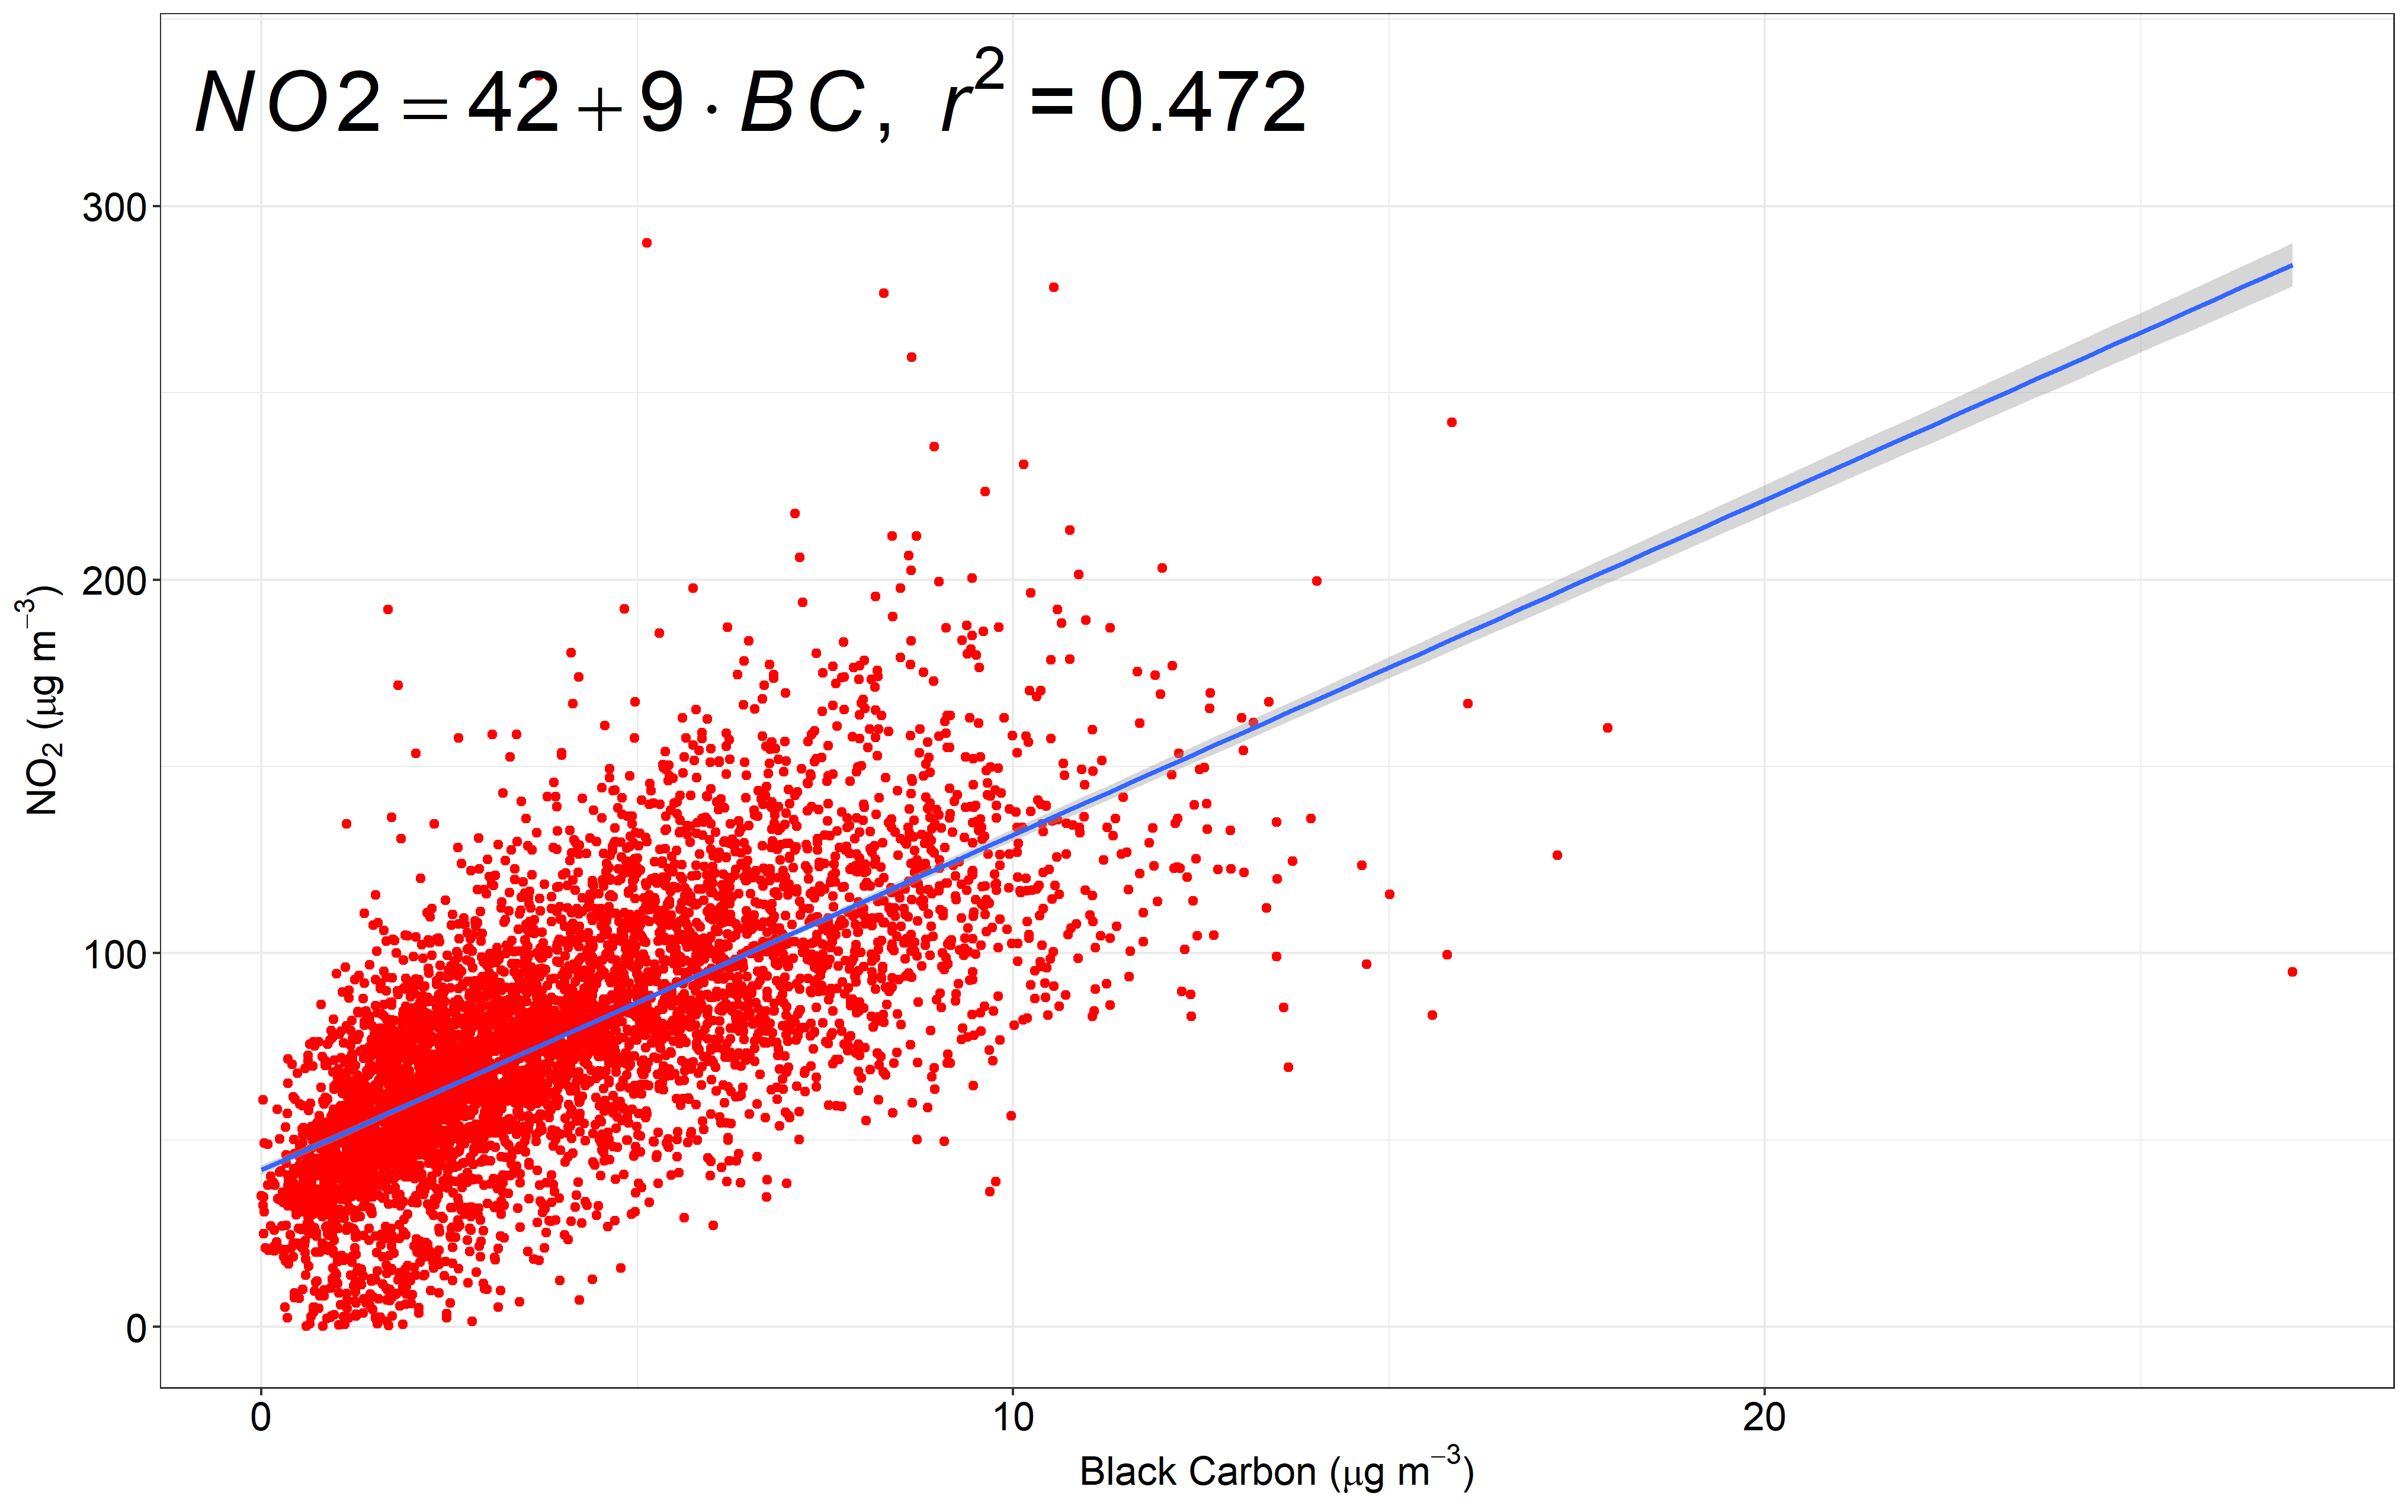
\includegraphics[scale=1]{images/black_carbon_no2_conversion.png}
\caption{Linear regression between black carbon and NO$_{2}$}
\label{fig:black_carbon_no2_conversion}
\end{figure}

This gave a conversion of NO$_{2}$ = 41 + 9.1 x BC, with a R\textsuperscript{2} of 0.474. A higher R\textsuperscript{2} would have been preferable to give more confidence to the BC-NO2 conversion process. This is again explored in the Discussion ( Section \ref{sec:4Discussion} ).

With regards to further sources of error in the evaluation of the LHEM using monitored data, it was presumed that the Microaeth AE51 was giving perfectly accurate readings of black carbon. Accepting that this is a limitation and in reality the device has been shown to have (relatively modest) measurement errors ( \cite{Cheng2013}, \cite{Viana2015} ).

A monitoring campaign was then completed over August and September, taking measurements on 28 cycling journeys between Kennington Park (51.484535, -0.109529) and Waterloo (51.505627, -0.111812) between 8am and 9am using the Microaeth AE51. The journey between Kennington Park and Waterloo was chosen due to convenience for the researcher and is purely arbitrary; the method could have been applied anywhere within the model domain.

%%%%%%%%%%%%%%%%%%%%%%%%%%%%%%
\subsection{Modelling journey exposure}
\label{subsec:modellingjourneyexposure}
%%%%%%%%%%%%%%%%%%%%%%%%%%%%%%

Using the CMAQ-UK air quality layer as an input I now modelled the exposure of the journey using the same methods as used in the LHEM from Chapter \ref{chap:the_lhem}. The route and concentrations along it are shown in Figure \ref{fig:dual_exposure_cycling} below.

\begin{figure}[H]
\centering
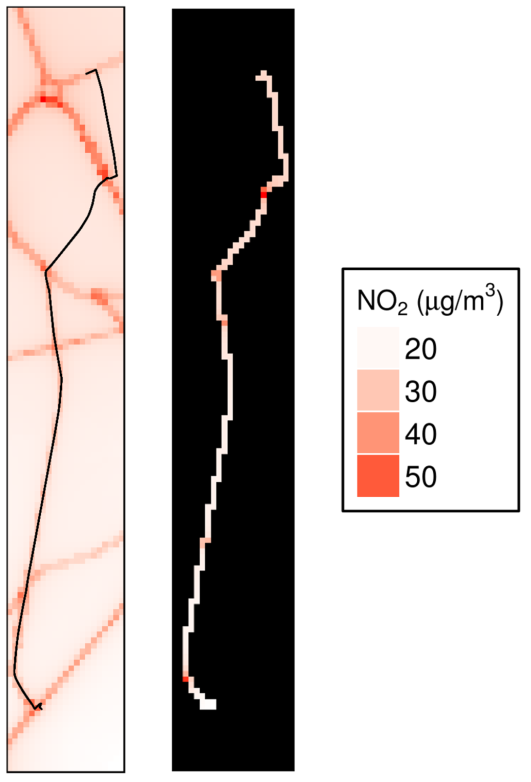
\includegraphics[scale=1]{images/dual_exposure_cycling.png}
\caption{Cycling journey between Kennington Park and Waterloo, overlain on modelled CMAQ-UK concentrations for 9am to 10am on weekdays in August to September}
\label{fig:dual_exposure_cycling}
\end{figure}

%%%%%%%%%%%%%%%%%%%%%%%%%%%%%%
\subsection{Data processing}
\label{subsec:dataprocessing}
%%%%%%%%%%%%%%%%%%%%%%%%%%%%%%

Before the measured exposure datasets could be compared to the modelled exposure of the same journey the following steps were completed:

\begin{itemize}
    \item Download raw CSV data from the Microaeth. Remove unnecessary columns and header meta-data.
    \item Import to R
    \item Divide black carbon concentrations by 1000 to convert into micrograms per metre cubed (for comparison with the NO$_{2}$)
    \item Manually fill in missing GPS data (device does not record position for first few minutes of operation, which was unknown at the time of data collection)
    \item Correct poor quality GPS data / drift by snapping GPS points to the nearest road segment (Shown in Figure 9)
    \item Create line segments instead of point positions.
\end{itemize}

\begin{figure}[H]
\centering
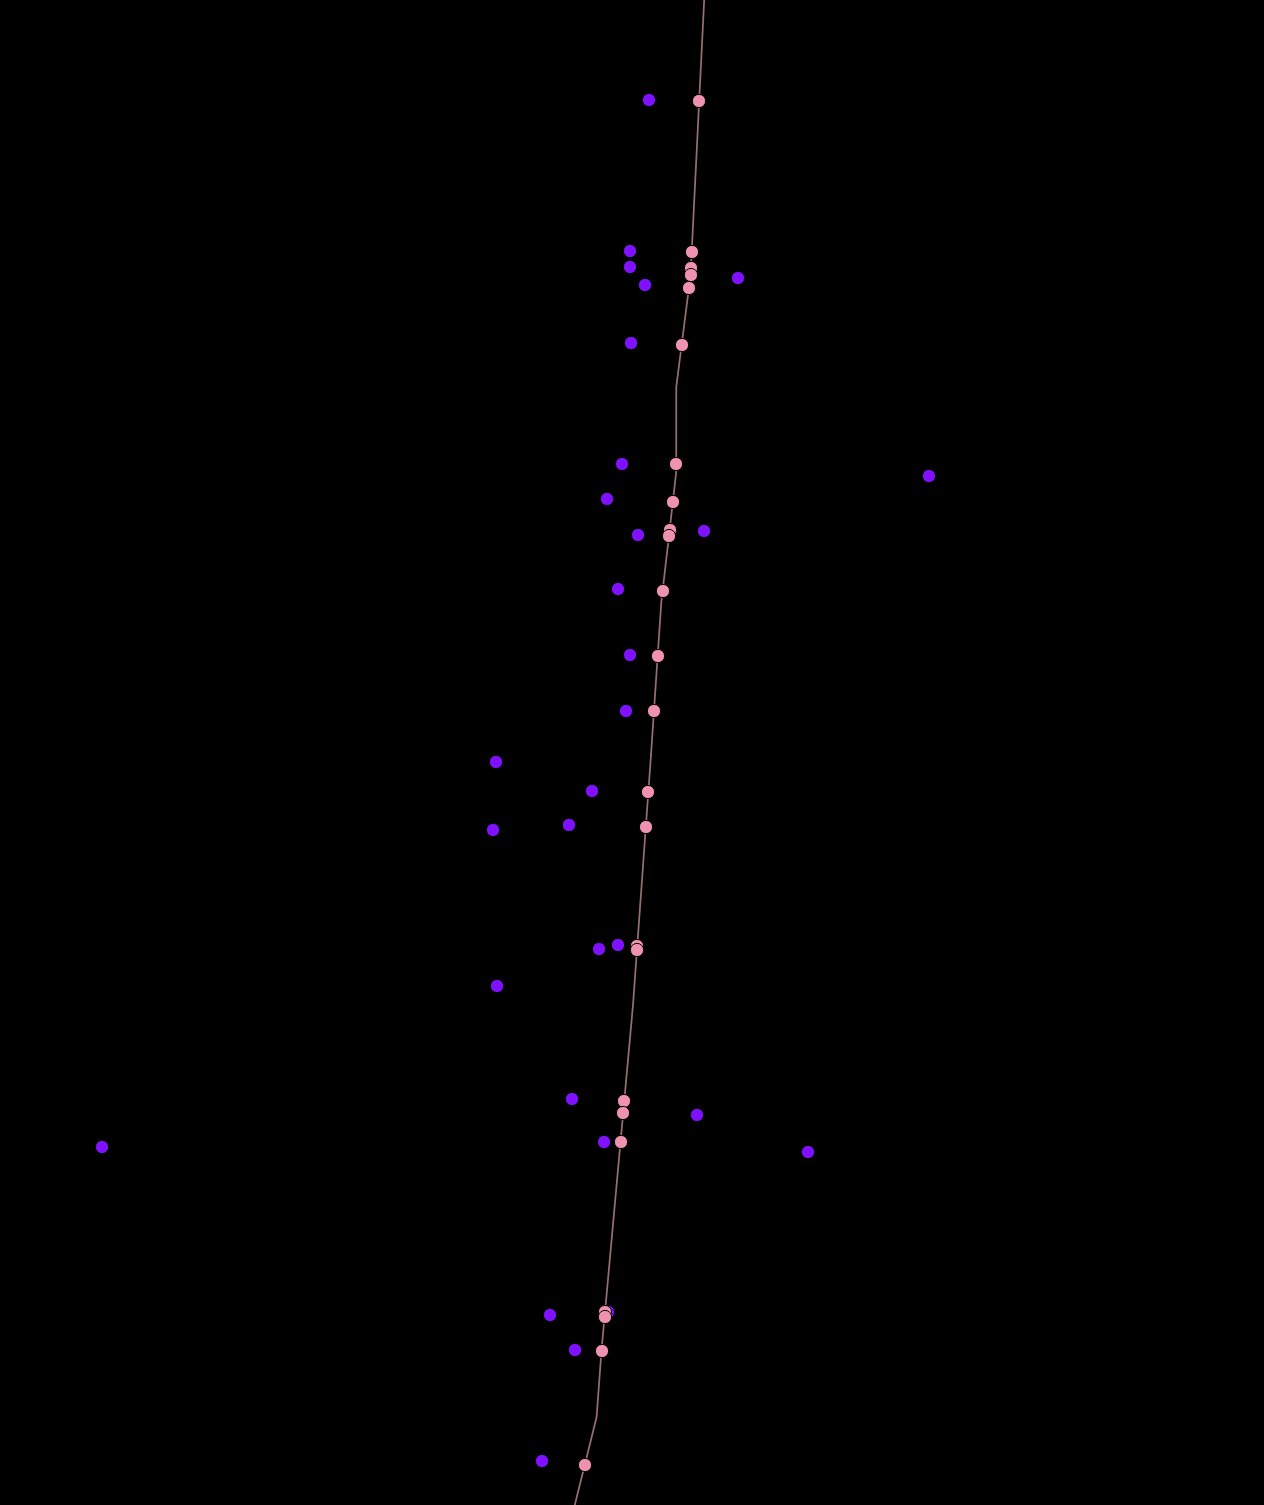
\includegraphics[scale=0.4]{images/snapping_cycle_to_road.png}
\caption{Locations of sampled BC concentrations along the cycle journey (purple), which have been snapped to the road (pink) to correct for GPS drift}
\label{fig:snapping_cycle_to_road}
\end{figure}

The final  step of creating line segments from points was required as the microaeth concentration that is stored each minute is at the end of one minute of sampling, meaning that the GPS position is the mean concentration from the previous minute of movement. To enable linking of this concentration with the CMAQ-UK grid squares during that period of movement, I created a SpatialLinesDataFrame line between each GPS point, and the previous GPS point in that journey, and assigned the concentration to that whole line.
The result of this processing of the monitoring data was 27 lines, stored as a SpatialLinesDataFrame (SLDF), split into segments of varying lengths, along the length of the journey from Kennington Park to the Waterloo. The start of one of the journeys is shown in Figure \ref{fig:cmaq_cycle_route_zoomed} below. Although not shown in the figure, the line has concentration attributes linked to it.

\begin{figure}[H]
\centering
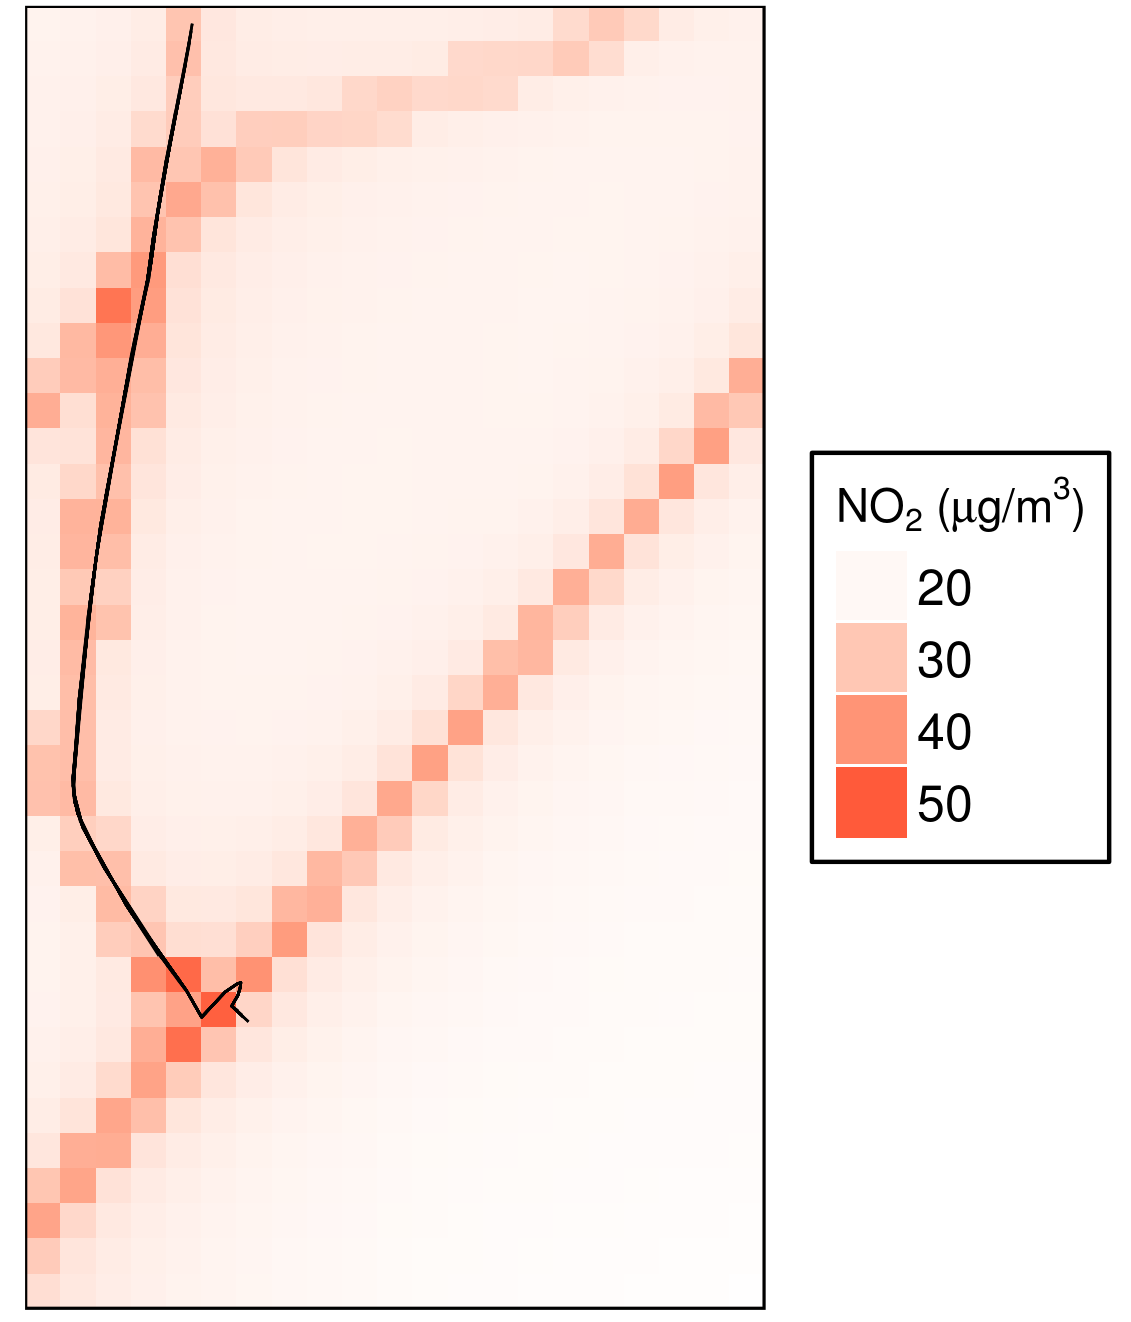
\includegraphics[scale=0.2]{images/cmaq_cycle_route_zoomed.png}
\caption{Start of a cycling journey from Kennington Park to Waterloo, cycle route shown by a black line, CMAQ model concentrations shown behind.}
\label{fig:cmaq_cycle_route_zoomed}
\end{figure}

Using the SLDF of measured concentrations, and the CMAQ-UK raster of modelled concentrations, two result datasets were now created:
\begin{itemize}
    \item \textbf{Concentration comparison}: The mean concentration from each journey, compared to the mean concentration of the grid cells that the journey intersected.
    \item \textbf{Spatial comparison}: For each grid cell the route intersected, I took the mean concentration from the 27 monitored lines that went through it. I then calculated the difference, by grid square, between the monitoring concentrations and the modelled concentrations and outputted this as a new raster file.
\end{itemize}

%%%%%%%%%%%%%%%%%%%%%%%%%%%%%%%%%%%%%%%%%%%%%%%%%%%%%%%%%%%%%%%%%%%%%%%%%%%%%%%%%%%
\section{Results}
\label{sec:4results}
%%%%%%%%%%%%%%%%%%%%%%%%%%%%%%%%%%%%%%%%%%%%%%%%%%%%%%%%%%%%%%%%%%%%%%%%%%%%%%%%%%%

%%%%%%%%%%%%%%%%%%%%%%%%%%%%%%
\subsection{Concentration comparisons}
\label{subsec:concentrationcomparisons}
%%%%%%%%%%%%%%%%%%%%%%%%%%%%%%

Figure \ref{fig:grouped_journey_boxplots} shows a boxplot summary graph of the 27 monitored journeys (right, black) compared to the modelled journey (left, red).

\begin{figure}[H]
\centering
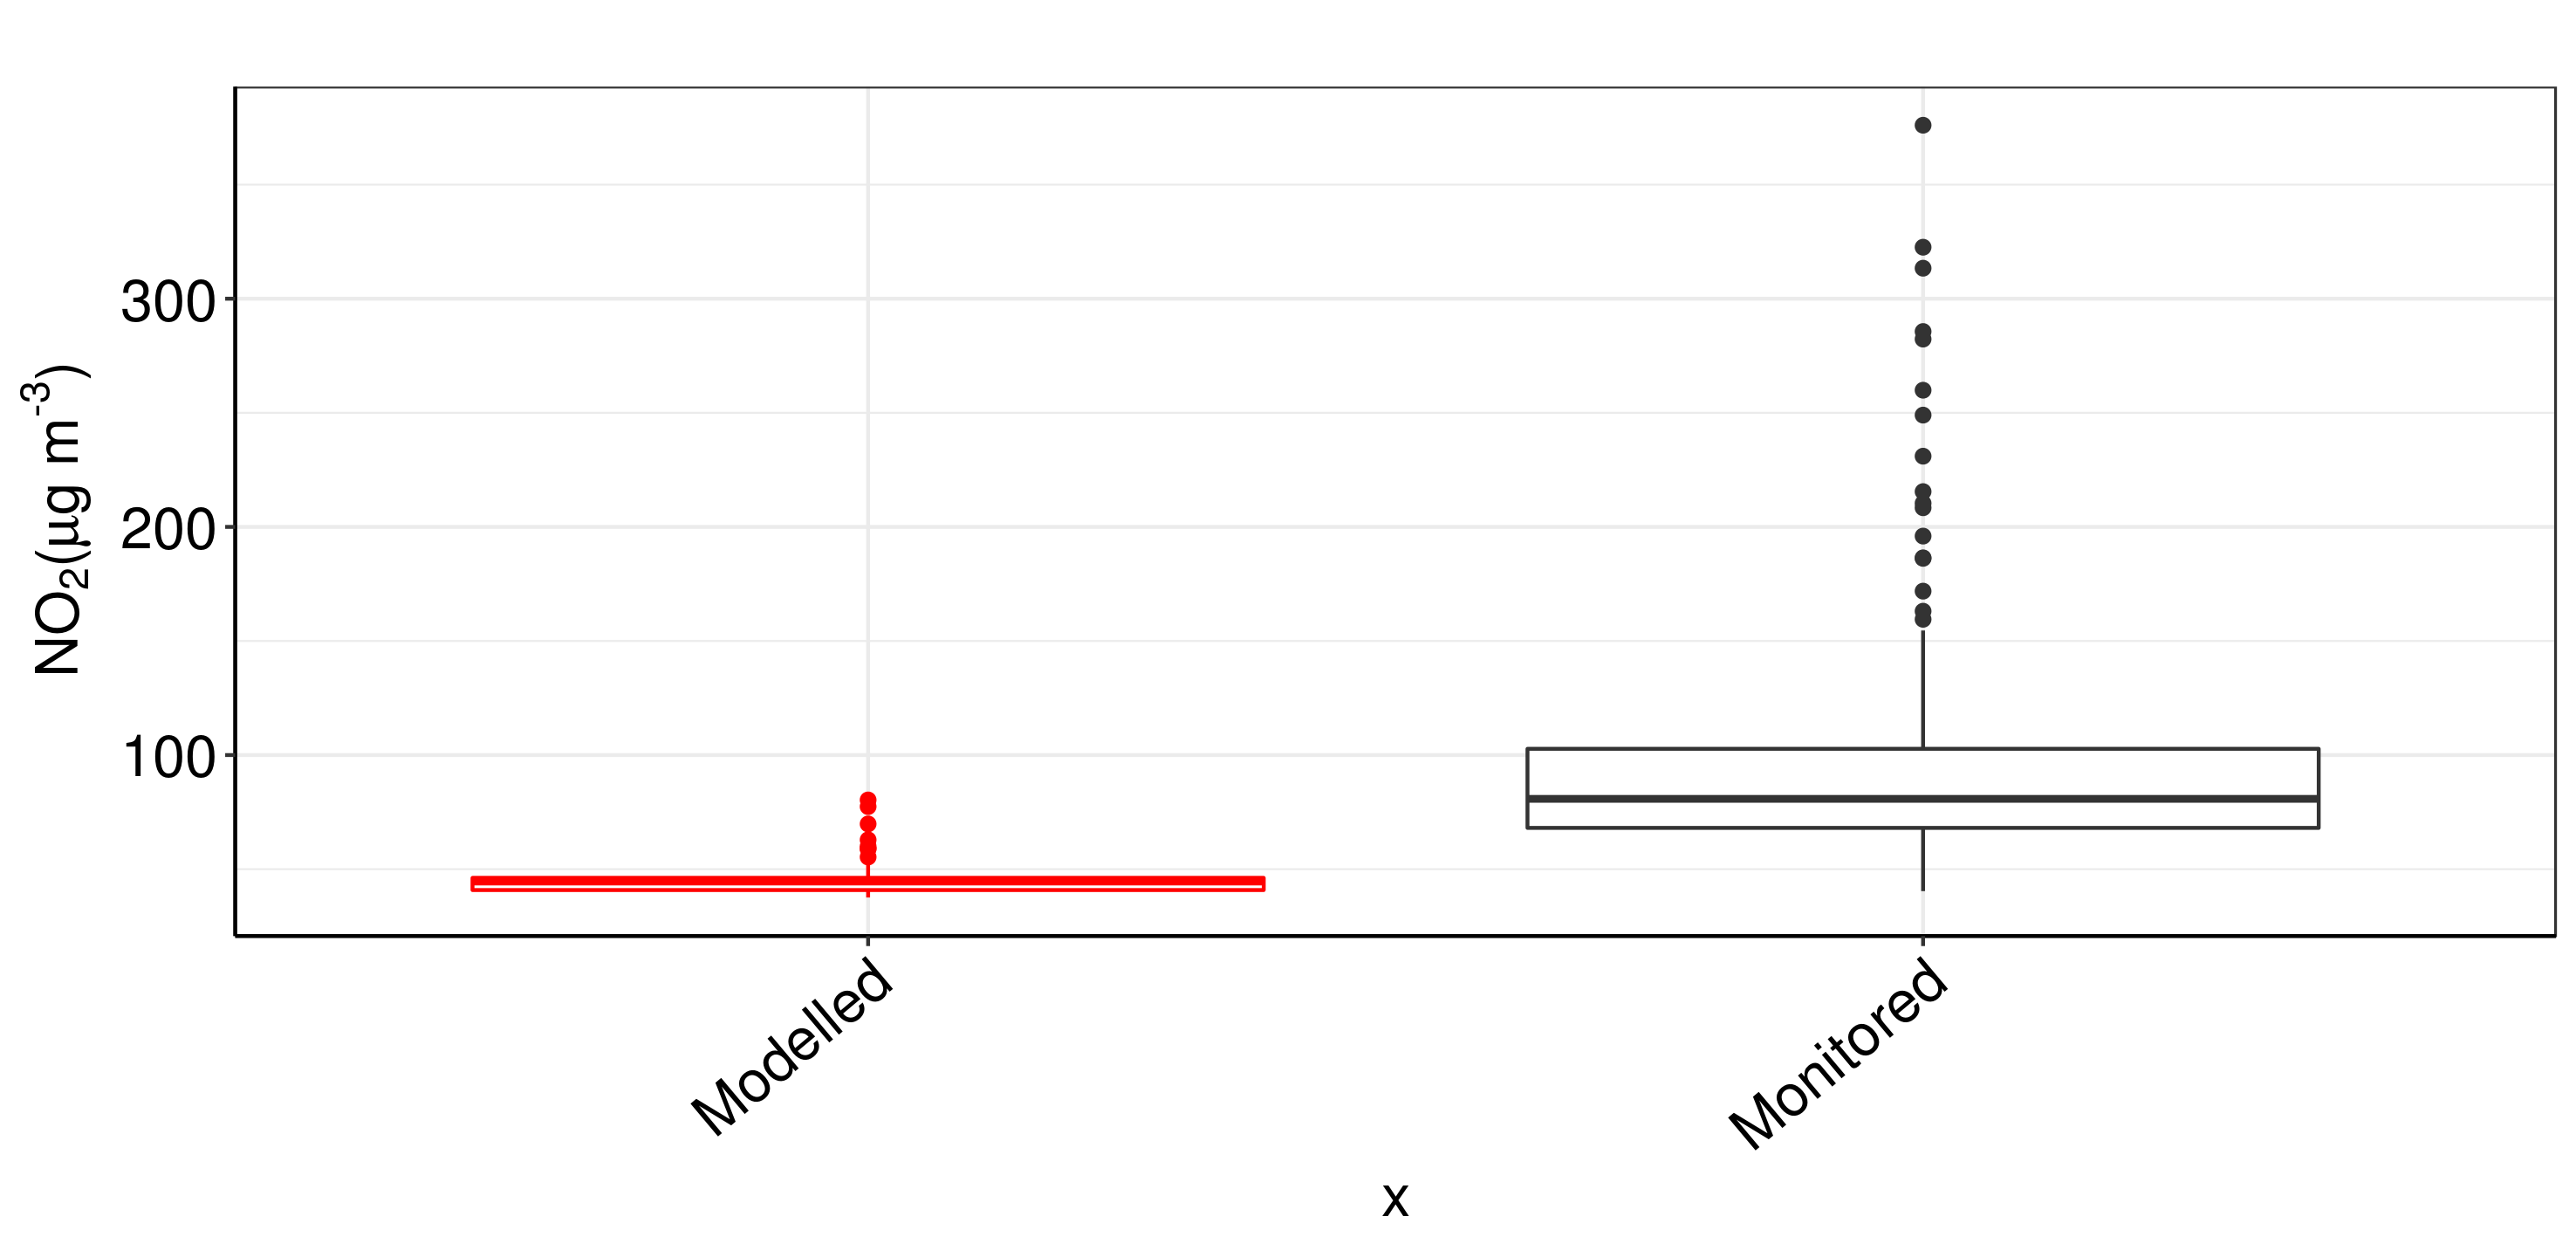
\includegraphics[scale=0.5]{images/grouped_journey_boxplots.png}
\caption{Box-plot of modelled cycling journey exposure compared to monitored cycling exposure}
\label{fig:grouped_journey_boxplots}
\end{figure}

From this summary plot we can see that in general the monitoring campaigns found higher concentrations than modelling the journey. When visualised individually (Figure \ref{fig:journey_boxplots}) we can see the variation more clearly. Noting that earlier we calculated that 27 repeat measurements were needed for a 80\% confidence interval and 30 $\mu \text{g m}^{-3}$ margin of error comparison, and should therefore really only be considering this data in aggregate form..

\begin{figure}[H]
\centering
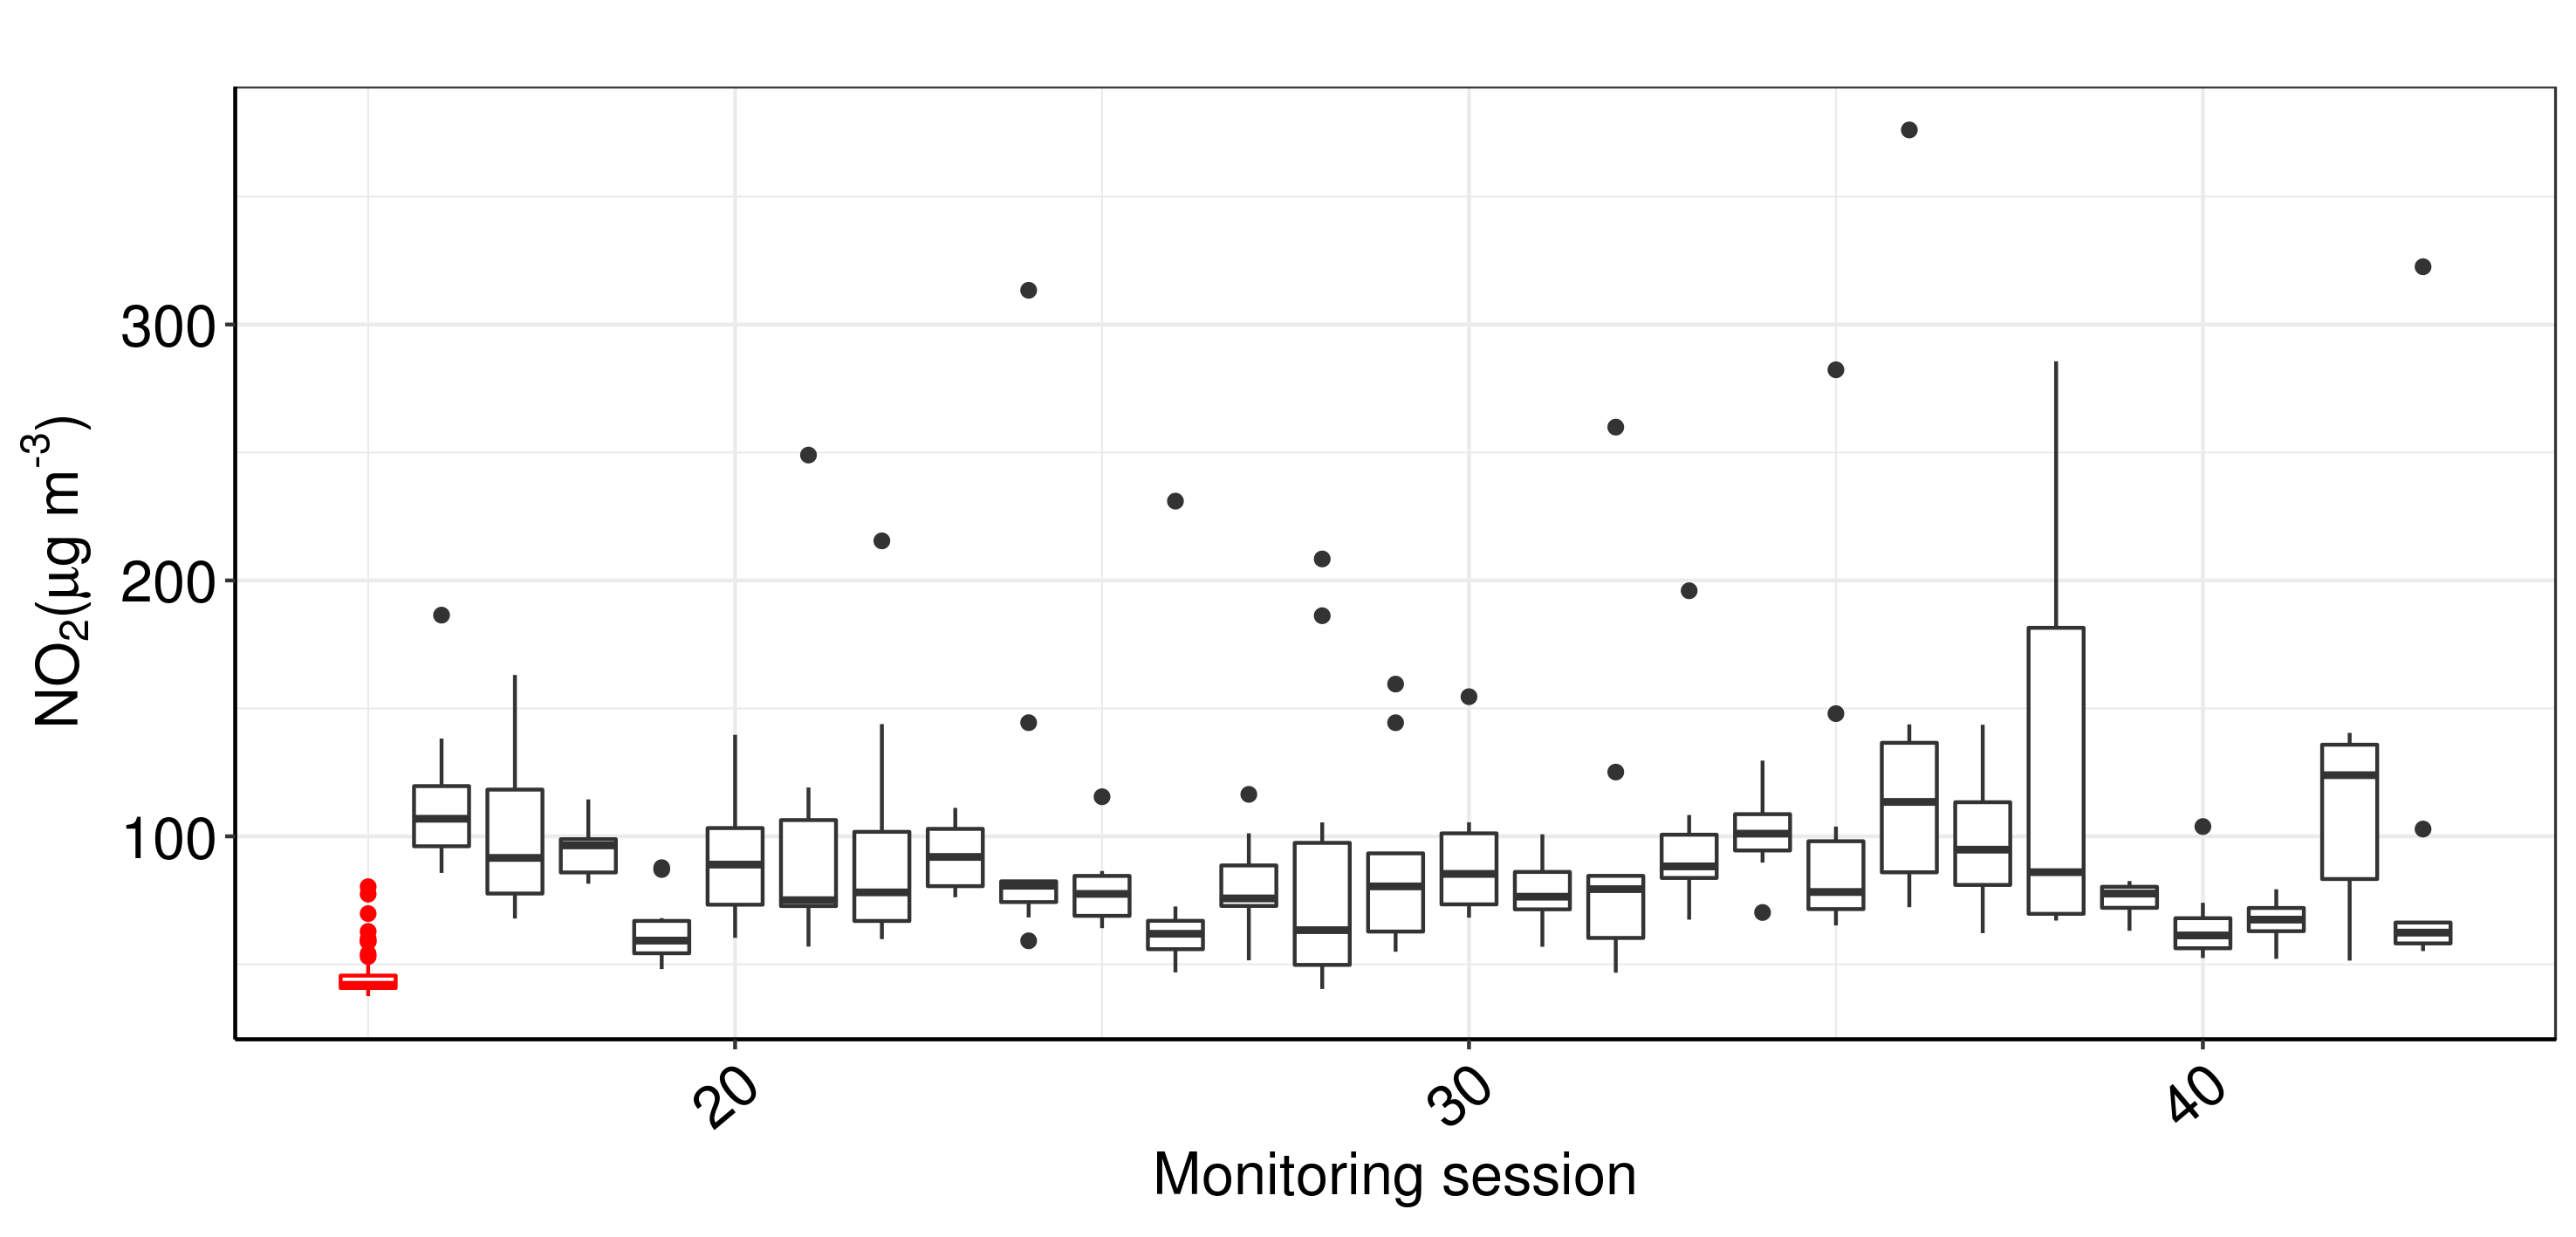
\includegraphics[scale=0.5]{images/journey_boxplots.png}
\caption{Box-plots of monitored cycling journeys (black) compared to the modelled cycling journey (red). Note that due to the device numbering system the sessions were numbered between 15 and 43, but there are not 43 sessions in the graph.}
\label{fig:journey_boxplots}
\end{figure}

Note that due to the device numbering system the sessions were numbered between 15 and 43, but there are not 43 sessions in the graph.

The summary statistics for these two datasets are shown in Table \ref{tab:modelled_monitored_cycling_summary}. Taking the raw monitored data against the modelled data, the lower boundaries of the datasets are similar, but the monitoring found mean and median concentrations approximately double that of the modelling, and the maximum monitored value is way in excess of the model. If we consider the monitored data, and include the allowable margin of error defined in the sample size calculation of 30 $\mu \text{g m}^{-3}$, then the agreement of the means at the lower boundary of the margin of error are much closer (64.19 $\mu \text{g m}^{-3}$ for monitored compared to 44.82 $\mu \text{g m}^{-3}$ for modelled). 

\begin{table}[H]
\centering
    \begin{tabular}{ | l | l | l |}
    \hline 
        & \bfseries{Modelled NO$_{2}$ $\mu \text{g m}^{-3}$} & \bfseries{Monitored NO$_{2}$ $\mu \text{g m}^{-3}$ (MOE)}                \\ \hline
     Minimum         & 37.58 & 40.35                \\ \hline
     1st Quartile    & 40.48 &  68.08               \\ \hline
     Median          & 44.57 & 80.81                \\ \hline
     Mean            & 44.82 & 94.19 (64.19-124.20) \\ \hline
     3rd Quartile    & 46.19 & 102.70               \\ \hline
     Maximum         & 80.33 & 376                  \\ \hline
    \end{tabular}
\caption{Comparison of measured and modelled exposure on the cycling journey}
\label{tab:modelled_monitored_cycling_summary}
\end{table}

%%%%%%%%%%%%%%%%%%%%%%%%%%%%%%
\subsection{Spatial Comparisons}
\label{subsec:spatialcomparisons}
%%%%%%%%%%%%%%%%%%%%%%%%%%%%%%

For reference, figure \ref{fig:cycling_journey} shows the journey from Kennington Park to Waterloo that we have been comparing.

\begin{figure}[H]
\centering
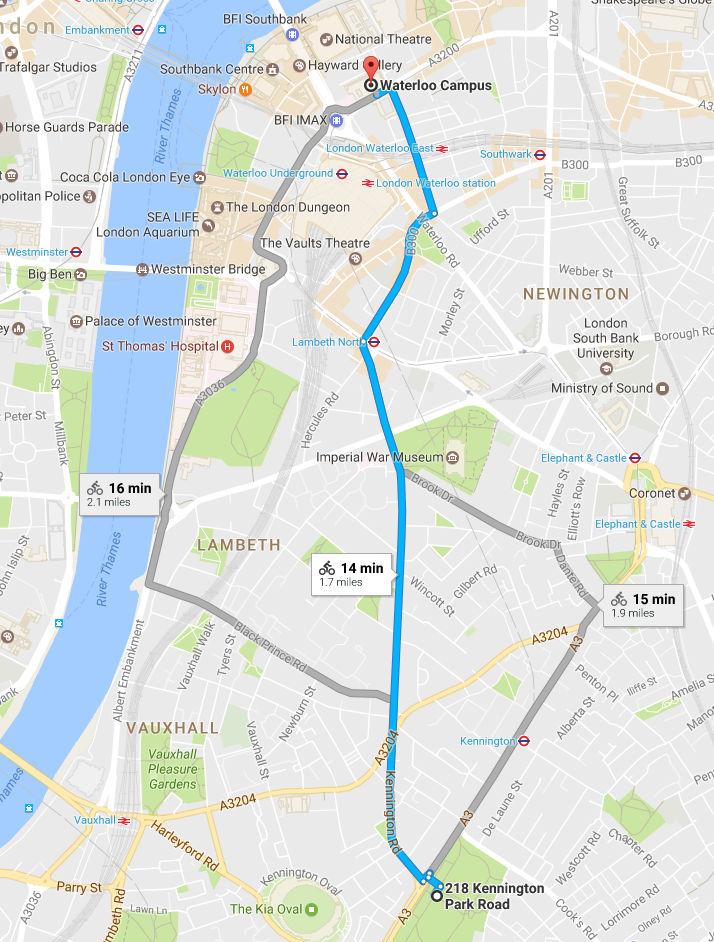
\includegraphics[scale=0.7]{images/cycling_journey.png}
\caption{Map of cycling route between Kennington Park and Waterloo}
\label{fig:cycling_journey}
\end{figure}

Figure \ref{fig:monitored_modelled_summary} below shows the monitoring data, the modelled data, and a comparison of the two on this route.

\begin{figure}[H]
\centering
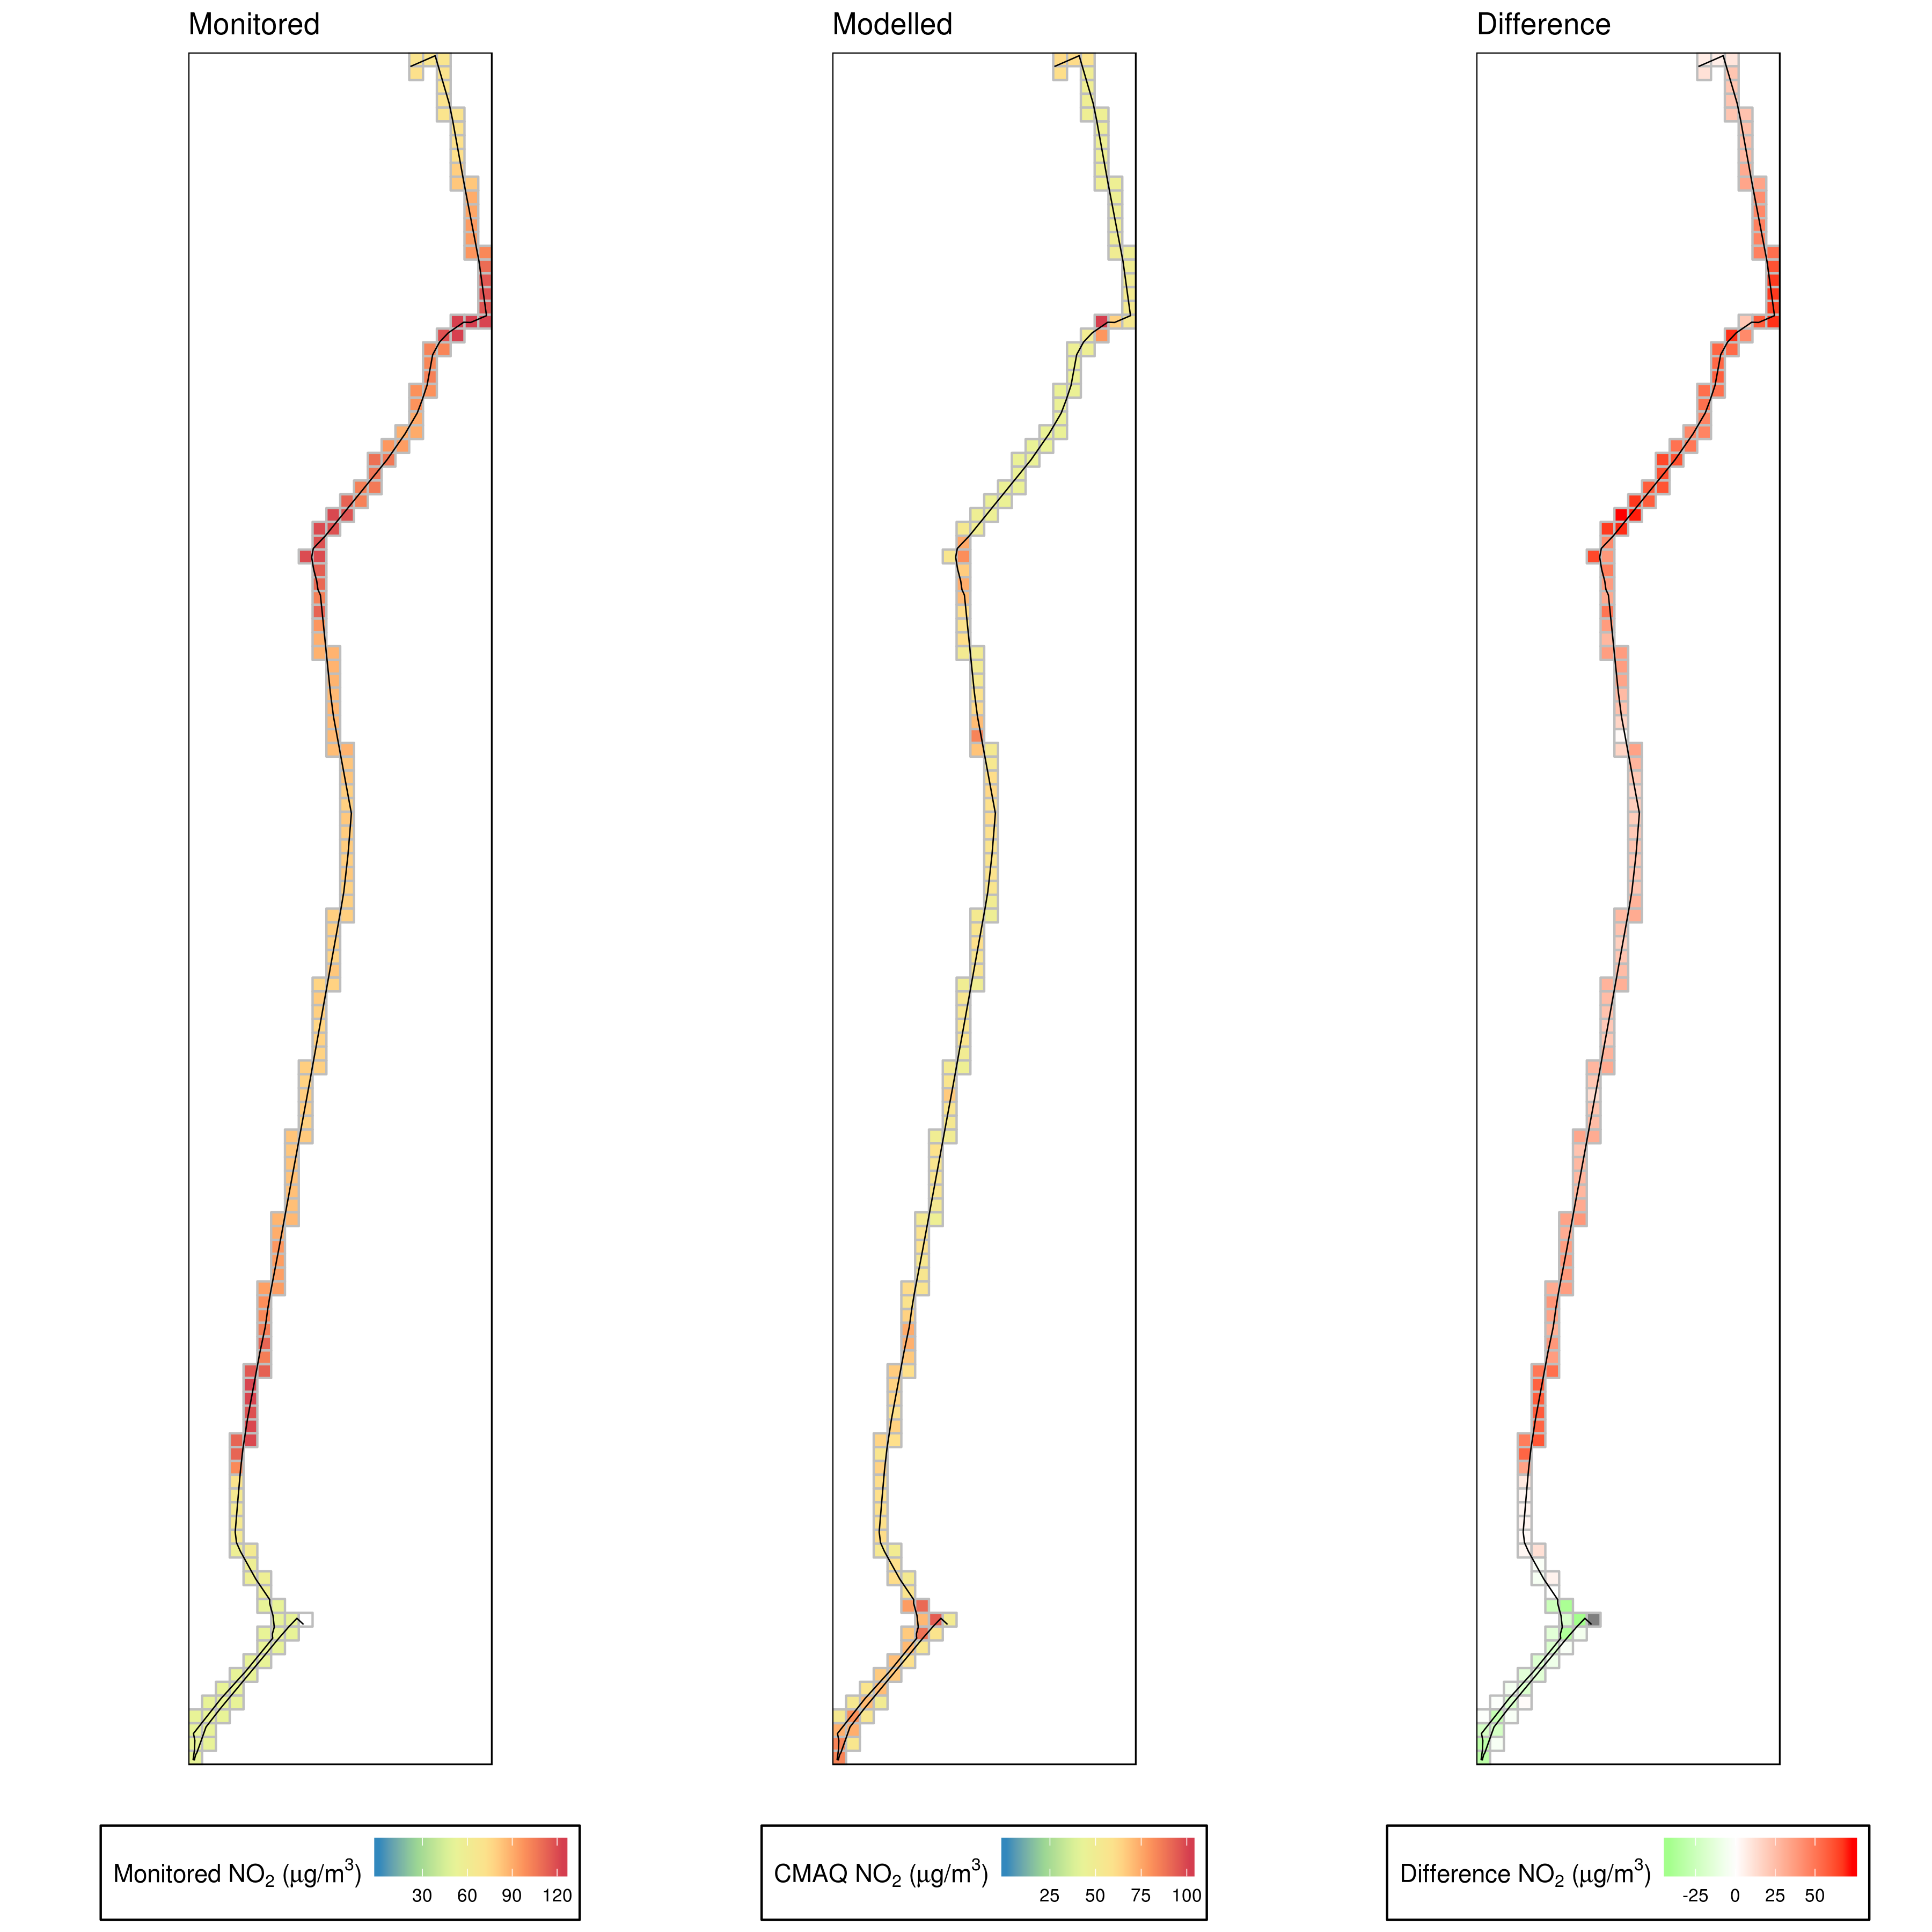
\includegraphics[scale=0.17]{images/monitored_modelled_summary.png}
\caption{Map of monitored, modelled and difference concentrations along the journey (NO$_{2}$ derived from black carbon)}
\label{fig:monitored_modelled_summary}
\end{figure}

By spatially comparing the results in this manner we can see that the monitoring campaign found the highest concentrations (> 100 $\mu \text{g m}^{-3}$) around the junction of Kennington Road and Kennington Lane (towards the South of the journey), near Lambeth North Station (a busy junction), and again near The Old Vic theatre (another busy junction). These locations of high concentrations are also found in the modelled data, but the difference against other stretches of the journey is not as large, and compared to the monitored data the concentrations are not as high. Considering the difference map (shown right in Figure \ref{fig:monitored_modelled_summary}), except for the first 5-10\% of the journey, most of the journey is underestimated by the model, between 0 and 25 $\mu \text{g m}^{-3}$ in each grid square. The largest differences are on Baylis Road, between Lambeth North Station and the Old Vic theatre, where the monitoring found concentrations to be up to 50 $\mu \text{g m}^{-3}$ higher. 

%%%%%%%%%%%%%%%%%%%%%%%%%%%%%%%%%%%%%%%%%%%%%%%%%%%%%%%%%%%%%%%%%%%%%%%%%%%%%%%%%%%
\section{Discussion}
\label{sec:4Discussion}

As discussed in the Background (Section \ref{sec:4background}), to my knowledge, there have not been any studies which have attempted to evaluate a dynamic approach to exposure in this manner. Studies have tended to measure certain micro-environments for a time-span often determined by practical constraints such as battery life, staff time and convenience; and then use these as empirical comparisons to their model outputs.
This piece of research was novel in that exposure was modelled, and then an attempt to evaluate the predictions (of an example journey) was undertaken by calculating how many personal monitoring samples would be needed, and then going out to collect that data. Despite various sources of possible error, this research demonstrated this as a possible process, and highlighted the difficulties of it. Reasonable ‘ball-park’ results were found, and clear spatial patterns were discernible. 

There were many issues and challenges to overcome whilst undertaking this evaluation that will have impacted the accuracy of the results. The main one being (mostly unavoidable) sources of error at each stage of the process. On the modelling side of the comparison CMAQ-UK has been shown to perform well when evaluated against monitoring sites, but it is far from perfect – the input the modelling uses for this chapter has NO$_{2}$ R values of 0.75. Against this, it was calculated that 27 samples would be needed to get a monitored concentration estimate that had a 30 $\mu \text{g m}^{-3}$ MOE (and 80\% CI). Black carbon samples were collected to do this, using a MA300 Microaeth, which has not yet been evaluated by academic literature (although previous models of similar equipment has R\textsuperscript{2} values of 0.8), and these data were converted to NO$_{2}$ using a linear regression with an R\textsuperscript{2} of 0.47. These multiple sources of error are bound to have confounded the results, but to what degree is uncertain. Post-hoc, it is not possible to go back and improve the CMAQ-UK model, or to collect more samples, or to improve the accuracy of the portable monitor, but it is interesting to reconsider the conversion process of black carbon to NO$_{2}$ from Figure \ref{fig:black_carbon_no2_conversion}. Visually the intercept of 41 looks high, and if this was theoretically changed to 0, then the measured concentrations would all be reduced, and the comparison between modelled and monitored would be much closer. Figures \ref{fig:grouped_journey_boxplots_new_intercept} and \ref{fig:monitored_minus_cmaq_route_cells_concs_zero_intercept} below show revised boxplot comparisons and spatial comparisons.

\begin{figure}[H]
\centering
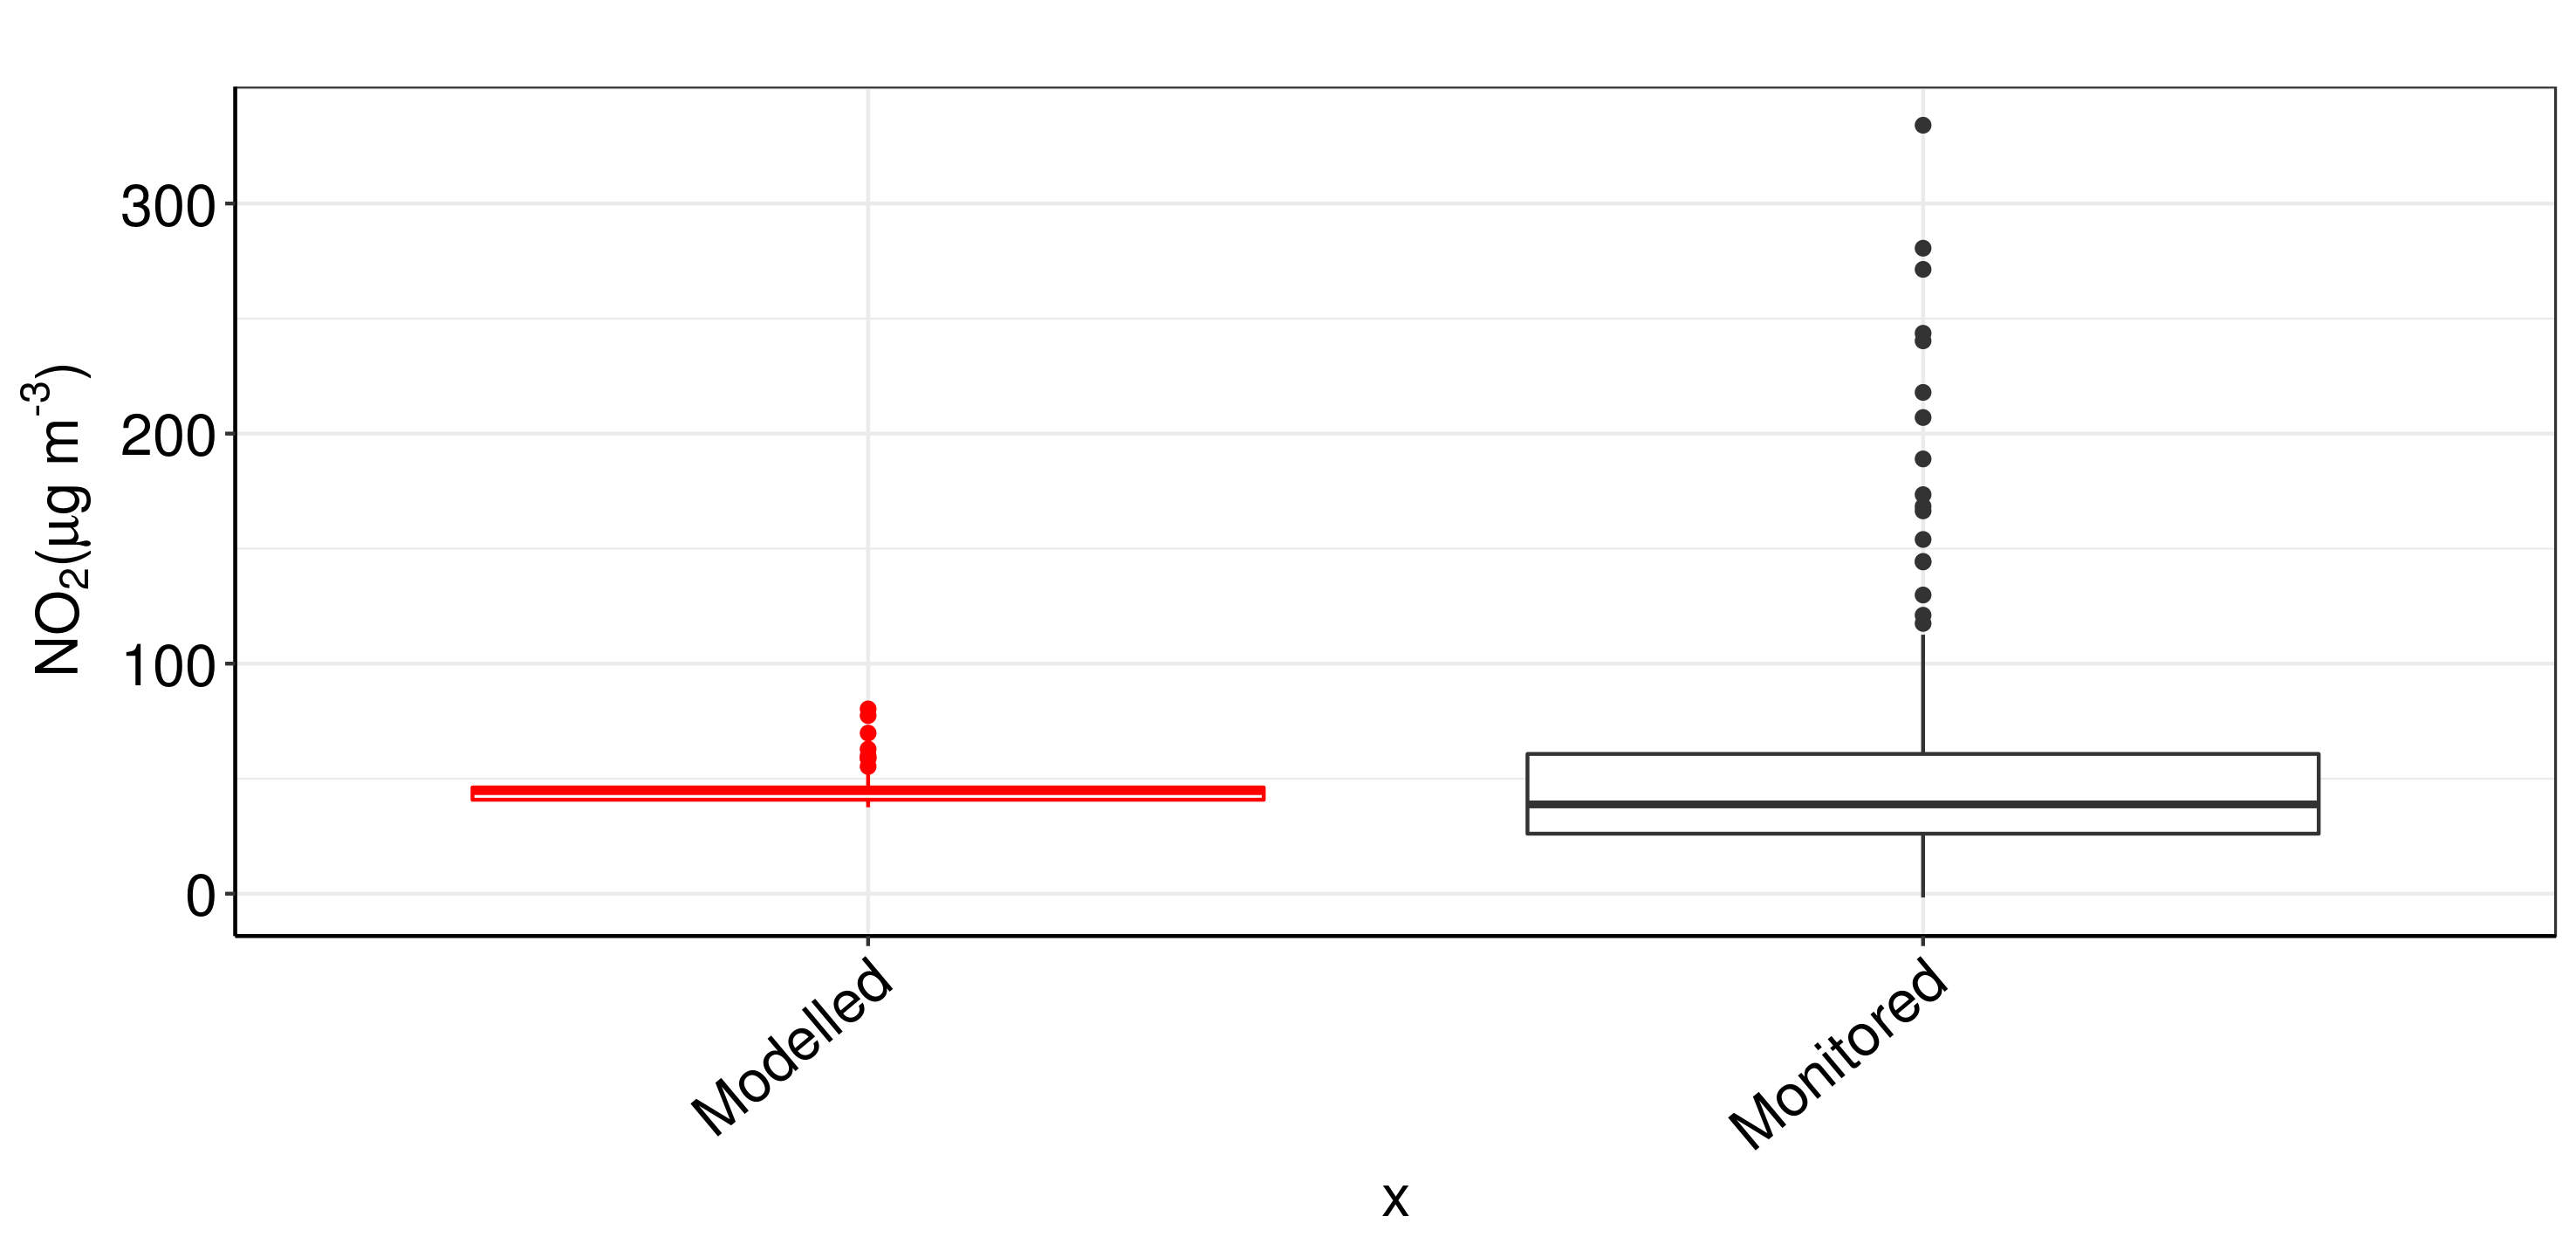
\includegraphics[scale=0.4]{images/grouped_journey_boxplots_new_intercept.png}
\caption{Boxplot comparison of modelled and monitored concentrations with an intercept of 0 between BC and NO$_{2}$}
\label{fig:grouped_journey_boxplots_new_intercept}
\end{figure}

\begin{figure}[H]
\centering
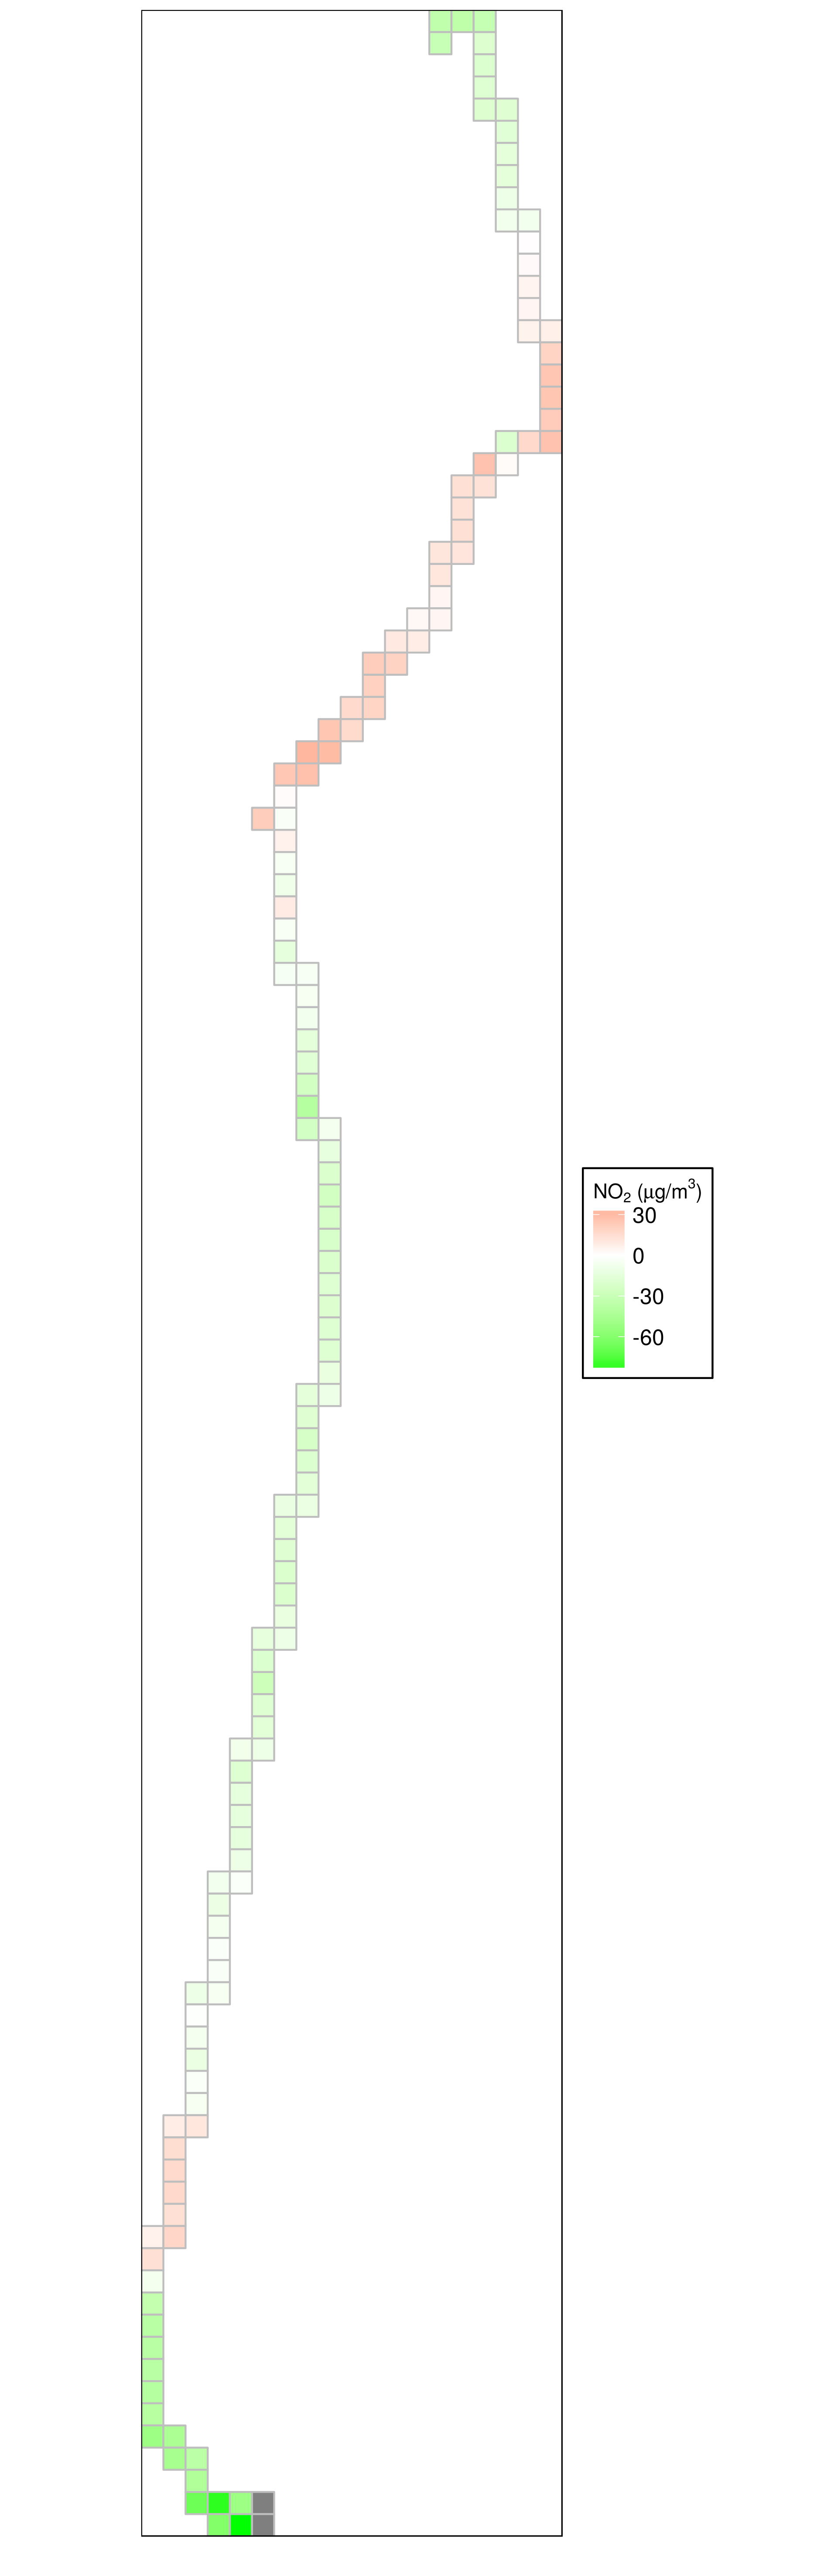
\includegraphics[scale=0.2]{images/monitored_minus_cmaq_route_cells_concs_zero_intercept.png}
\caption{Spatial comparison of modelled and monitored concentrations with an intercept of 0 between BC and NO$_{2}$}
\label{fig:monitored_minus_cmaq_route_cells_concs_zero_intercept}
\end{figure}

Putting measurement errors and modelling errors aside, there are practical improvements that could be implemented in repeating this work which might lead to improved results. The most notable being the sample size. If the journey had been shorter, or more researchers were available, it would have been possible to collect a much larger number of samples, which according to the sample size calculations would have increased the reliability of the results. A more practical long-term approach to evaluating air quality model inputs to a hybrid exposure model could be to fix reliable portal monitors to cars or public transport and increase sample size in this manner. For example, mobile monitors might be attached to the outside of a fleet of No.59 buses which run along the route I cycled, meaning each grid square would be sampled 10-15 times between 9am and 10am, resulting in 400-500 measurements over the same time period. Indeed, our group are already trialling a similar method, but with the monitors inside a bus to measure the changes in passenger exposure from the electrification of a bus route in London.

Focusing on the equipment, an unforeseen issue in collecting the monitoring data was a mismatch between cycling speed, the resolution of the CMAQ-UK grid squares, and the temporal resolution of the Microaeth MA300. I wanted to measure concentrations in each grid square along a route, but as the Microaeth was set to 1-minute resolution, the grid squares are 20m by 20m, and typical cycling speed is 15 km/h (or 250 metres per minute), this meant that each minute of Microaeth data covered 250/20 = 12.5 grid squares. Repeating this experiment, a researcher could calculate the sampling rate of the device based upon the likely speed of the movement, and the air quality model resolution it will be compared to, as per equation \ref{eq:sampling_rate_equation}

\begin{equation}
  sampling rate_{(minutes)} = \frac{AQ_{(metres)}}{speed_{(metres/minute)}}
  \label{eq:sampling_rate_equation}
\end{equation}

Though this would of course be constrained by the settings available in the sampling device.

Within the GIS and data processing section of this work, the main issue was the lack of accuracy of the GPS points that were output from the device, how to snap these appropriately to roads (presuming an available roads dataset), and how to link this to CMAQ-UK concentration grid squares for analysis. This was time-consuming and required manual editing at times. Automating this for a large scale campaign would be challenging but necessary. Junctions were a particular difficulty, for instance snapping GPS points at a left-turn always means that the point is snapped to part of the road either side of the junction and never at the actual junction itself (Figure \ref{fig:gps_snapping_error}); which might be where the highest concentrations occur and the researcher is most interested.

\begin{figure}[H]
\centering
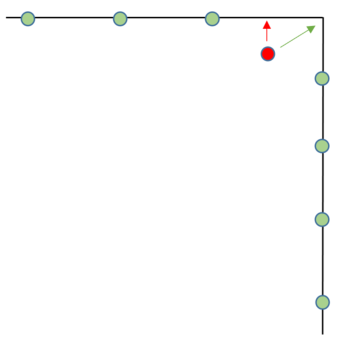
\includegraphics[scale=0.7]{images/gps_snapping_error.png}
\caption{Accurate GPS points shown in green, GPS error shown in red. Correction should move the point to location shown by green arrow, but simple ‘snapping’ will move it to direction of red arrow.}
\label{fig:gps_snapping_error}
\end{figure}

%%%%%%%%%%%%%%%%%%%%%%%%%%%%%%%%%%%%%%%%%%%%%%%%%%%%%%%%%%%%%%%%%%%%%%%%%%%%%%%%%%%
\section{Conclusions}
\label{sec:4conclusions}

The main conclusions from this chapter are method-orientated, rather than definitive answers about the reliability of a hybrid exposure method. The amount of data collection and data processing were both extremely onerous in order to even evaluate one journey, requiring skills in data processing, GIS, statistics and personal monitoring. To repeat this method on a larger scale initial consideration should be given to the monitors that are going to be used, and in which possible transport modes, to ensure that they provide a high enough temporal and spatial resolution for alignment with the modelled air quality being used by the exposure modelling. Similarly, testing the monitors extensively to ensure that the parameters required are output immediately rather than taking a short period of time to internally calibrate themselves when turned on (as I unfortunately found with the GPS sensor of the Microaeth which led to hours of manual correction).
The sample size calculations here demonstrated a method (given a fixed reliable ‘base’ dataset) to estimate the number of samples that are required to arrive at monitored concentrations that have a low margin of error and high confidence. For this piece of research, it was calculated that over 1,000 measurements would have been needed to give a low margin of error with high confidence, but it is worth noting that this figure depends on the pollutant of interest, the base data, and the geographical area. It could be much higher or lower. 
Regarding results rather than method, I found that the CMAQ-UK NO$_{2}$ model used as an input to the London Hybrid Exposure Model is underestimating concentrations for the journey I chose. Whether this can be extrapolated to draw wider conclusions about the model are unclear. The findings have large caveats due to multiple, mostly unavoidable, sources of error in the method e.g. the black carbon to NO$_{2}$ conversion and sample size, that require fuller exploration of their impact and propagation.

%%%%%%%%%%%%%%%%%%%%%%%%%%%%%%%%%%%%%%%%%%%%%%%%%%%%%%%%%%%%%%%%%%%%%%%%%%%%%%%%%%%